\section{Implementation}
\label{sub:Implemenation}
The following sections describe, how the implementation of the automatic room recognition was achieved. Basically it is split into three parts, later called workflows. Each workflow is a combination of algorithms, which solves a different problem.

Every section will describe why and how the algorithm is implemented and what the results of the implementation was.

\subsection{Workflow 1}
\label{sub:workflow1}
This section describes the first combination of algorithms that was implemented to try and achieve room detection. It is based on research of the paper by Ahmed, Liwicki, Weber and Dengel \citep{mace_valveny_loctea_tabbone_2010} to find the walls in an image with a Hough transformation. To then detect the rooms, the idea was to detect them with a watershed algorithm. This algorithm is used by several projects on the internet, on the context of room segmentation. The general idea, how this algorithm is supposed to work and what problems were found, are described in this section.

\begin{figure}[H]
	\centering
	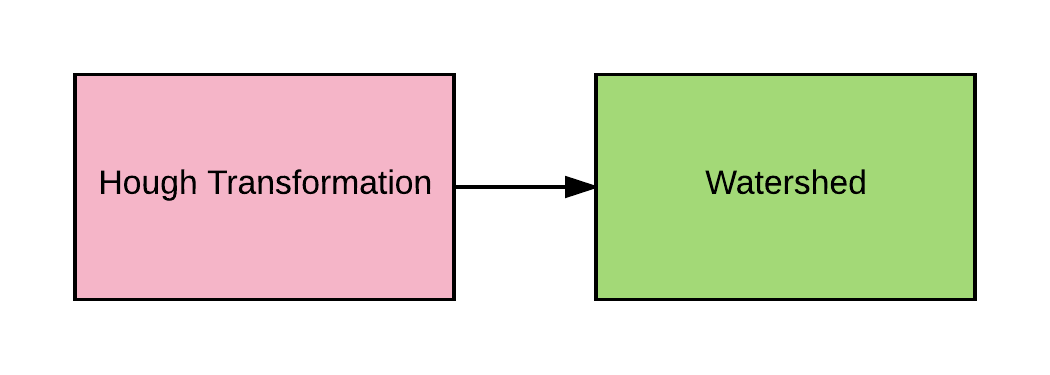
\includegraphics[width=0.8\textwidth]{Workflow1Flowchart}
	\caption{Workflow 1 flowchart.}
	\label{fig:Workflow1Flowchart}
\end{figure}

\subsubsection{Hough transformation}
This implementation is based on the fact that the Hough transformation will find long lines on an image. These lines will usually be the walls. Cleaned up images of architectural floor plans were used to start off. This was done to remove noise on plans so the walls could be extracted easily.

As described in section~\ref{subsubsec:Hough transformation}, the Hough transformation finds straight lines on an image. Long straight lines on a floor plan are usually the walls, therefore the Hough transformation is supposed to detect them on the plan. As a precondition for the Hough algorithm, a binary image is needed. To create this binary image, we use the Canny Edge detection algorithm by OpenCV. Wherever it detects an edge, the pixels will be white, all other pixels will be black. There will be two edges for each wall, one where the background changes to the wall and the other, where the wall ends and the background starts again. To then detect the lines, the Hough transformation by OpenCv, called HoughLines, was used first. It finds all the suspected lines and returns it in an array represented with the $(r,\theta)$ orientation representation. The problem with this implementation was, that this just represents the orientation and location of the line but not its size.
As a replacement HoughLinesP was used. It does the exact same, but additionally calculates where those lines actually are. The resulting array returns the actual starting and ending position of the lines. 

There were several problems with that algorithm. The algorithm separated a wall line into a lot of small lines. To retrieve the actual wall there would have to be additional computation that connects those several small parts into one big line. As an addition, due to no preprocessing, what was left as a wall, were the actual outlines of the original walls. Therefore, any wall was represented by two parallel lines. This would have led to additional effort. Before any of those efforts were made, a different algorithm was found that showed more promising results. Therefore the optimization of this algorithm was not pursued further.

  
\subsubsection{Watershed}
The idea to find the different rooms within the floor plan, was to run the watershed algorithm on the image (Section~\ref{subsub:watershed}). It is a flood filling algorithm that starts at given starting points and extends its area, until it meets a wall or a different flood from an other starting point. A further explanation will be done in section~\ref{subsubsub:watershed}, as it was actually implemented and used in our second workflow.

\subsection{Workflow 2}
\label{sub:workflow2}
This section describes the second workflow and what algorithms it is composed of. It is a mix of the work of Sébastien Macé and Peter Dawkins and Hervé Locteau and Salvatore Tabbone~\citep{mace_valveny_loctea_tabbone_2010} and the experiences we made with the first workflow~\ref{sub:workflow1}. What it does, is it removes any noise on the floor plan first with morphological operations, like erosion and dilation. This is followed up with a room detection algorithm that, in the end, uses the watershed algorithm to determine the rooms. In contrast to the first workflow, where the preprocessing for the watershed was not done sufficiently, this algorithm improved that. After optimizing this workflow, it was the first workflow that showed actual potential and was able to detect the rooms and therefore solve the given problem.


\begin{figure}[H]
	\centering
	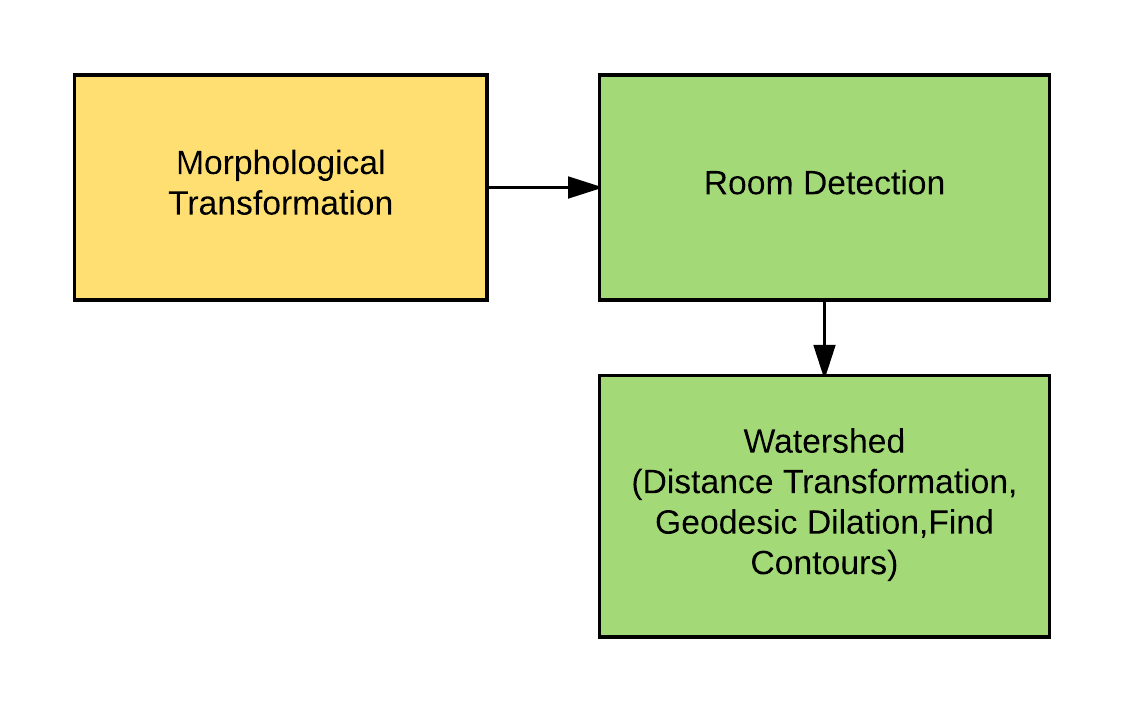
\includegraphics[width=0.8\textwidth]{Workflow2Flowchart}
	\caption{Workflow 2 flowchart.}
	\label{fig:Workflow2Flowchart}
\end{figure}

\subsubsection{Noise removal}
All of the following topics in this section are used to remove or add specific information from our image. The idea is to standardize all incoming floor plans regardless of what "noise" is around in the basic floor plan. Noise is anything that is of no importance to all the following algorithms. This contains elements such as "personal-property" (cars, pianos, etc.) as well as text or any lines to show dimensions on the plan. The idea would be that most of this noise is erased by the user in advance. But it is practically impossible to remove all the noise beforehand, due to it being so time intensive. It would ruin all the benefits of the algorithm, which uses less time than doing everything by hand.

\paragraph{Morphological transformation}
\label{sub:MorphologicalTransformation}

The basic principle to remove noise is erosion and dilation. How the algorithm is processed is explained in section~\ref{subsubsec:Erosion and Dilation}.
The purpose of both of those algorithms in this project is to remove any information on the starting picture, to get a picture containing only the walls. This works due to the fact that usually the walls are the thickest lines on the floor plan. It is a simple heuristic to extract the walls and is according to the method other papers use (see \citep{ahmed_liwicki_weber_dengel_2012}).

This project always uses a combination of erosion and dilation to retain the original place of all the walls. The size of the rooms would differ from the original size if we did not do the same dilation after an erosion and vice versa. This would render all the results useless, since a basic requirement is to find the actual room polygon. There are two ways to use noise removal as a combination of erosion and dilation. 

\begin{description}[style=nextline]
	\item[Erosion first] This removes thin lines from the image. Those are non walls and therefore of no importance to the output image. The dilation brings the remaining lines back to its original size.
	\item[Dilation first] This extends all lines and combines any lines that are close to each other. The erosion following then creates one line out of the bunch. This is used to combine walls that are created out of several thin lines into one thick line.
\end{description}

Both of those combinations are used in the morphological transformation class. First used is the "dilation first" transform to combine the walls out of several lines into one. This results in all the walls being one thick line instead of a multitude of small lines. This guarantees that all walls are thick lines and won't get erased with the "erosion first" transform. This is now followed with the "erosion first" transform to erase all the other lines besides the walls. 

\begin{figure}[H]
	\centering
	\subfloat[Original image.]{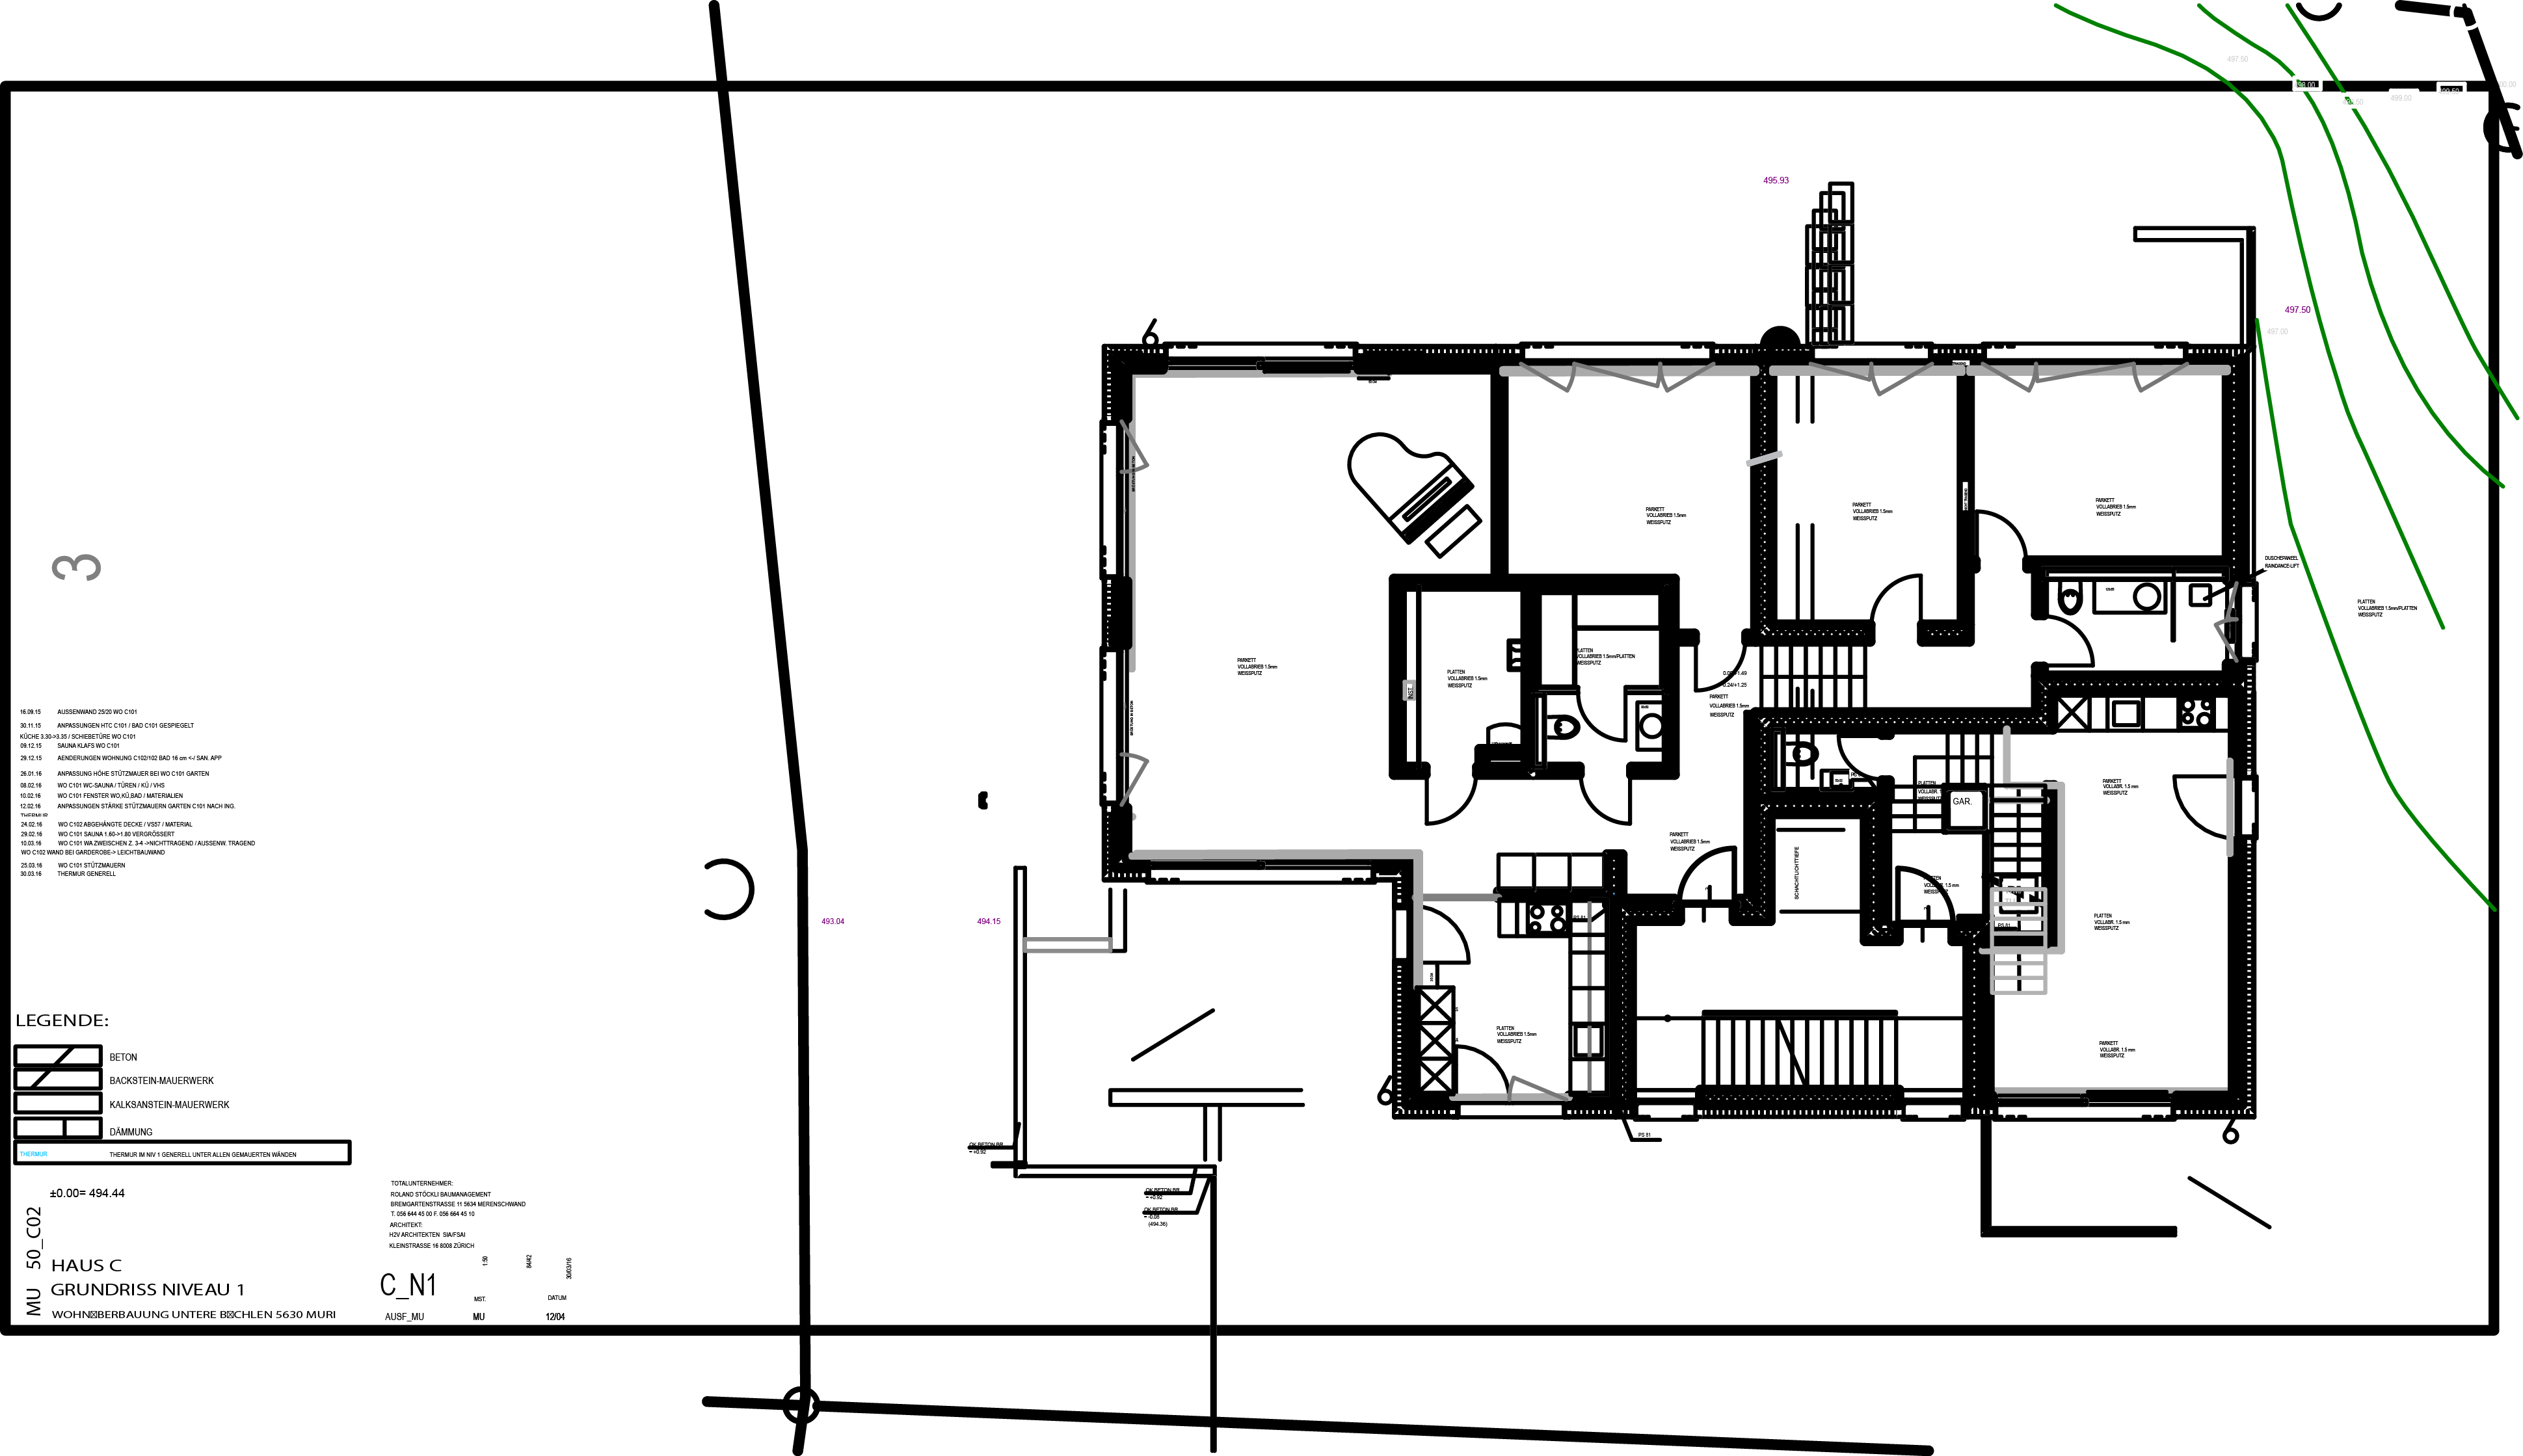
\includegraphics[width=0.5\textwidth]{A_N1.png}\label{fig:A_N1}}
	\hfill
	\subfloat[Image after noise removal.]{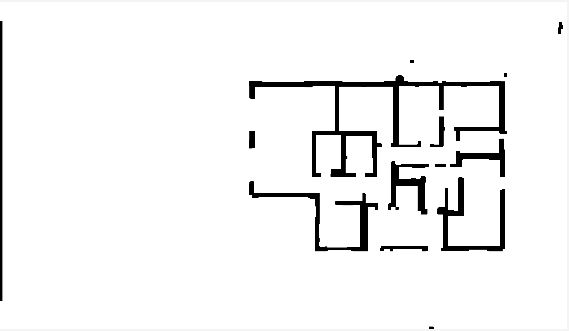
\includegraphics[width=0.4\textwidth]{morphtransuncleaned.jpg}\label{fig:A_N1_Morph}}
	\caption{Before and after of an uncleaned floor plan with noise removal. }
\end{figure}

\begin{figure}[H]
	\centering
	\subfloat[Original image.]{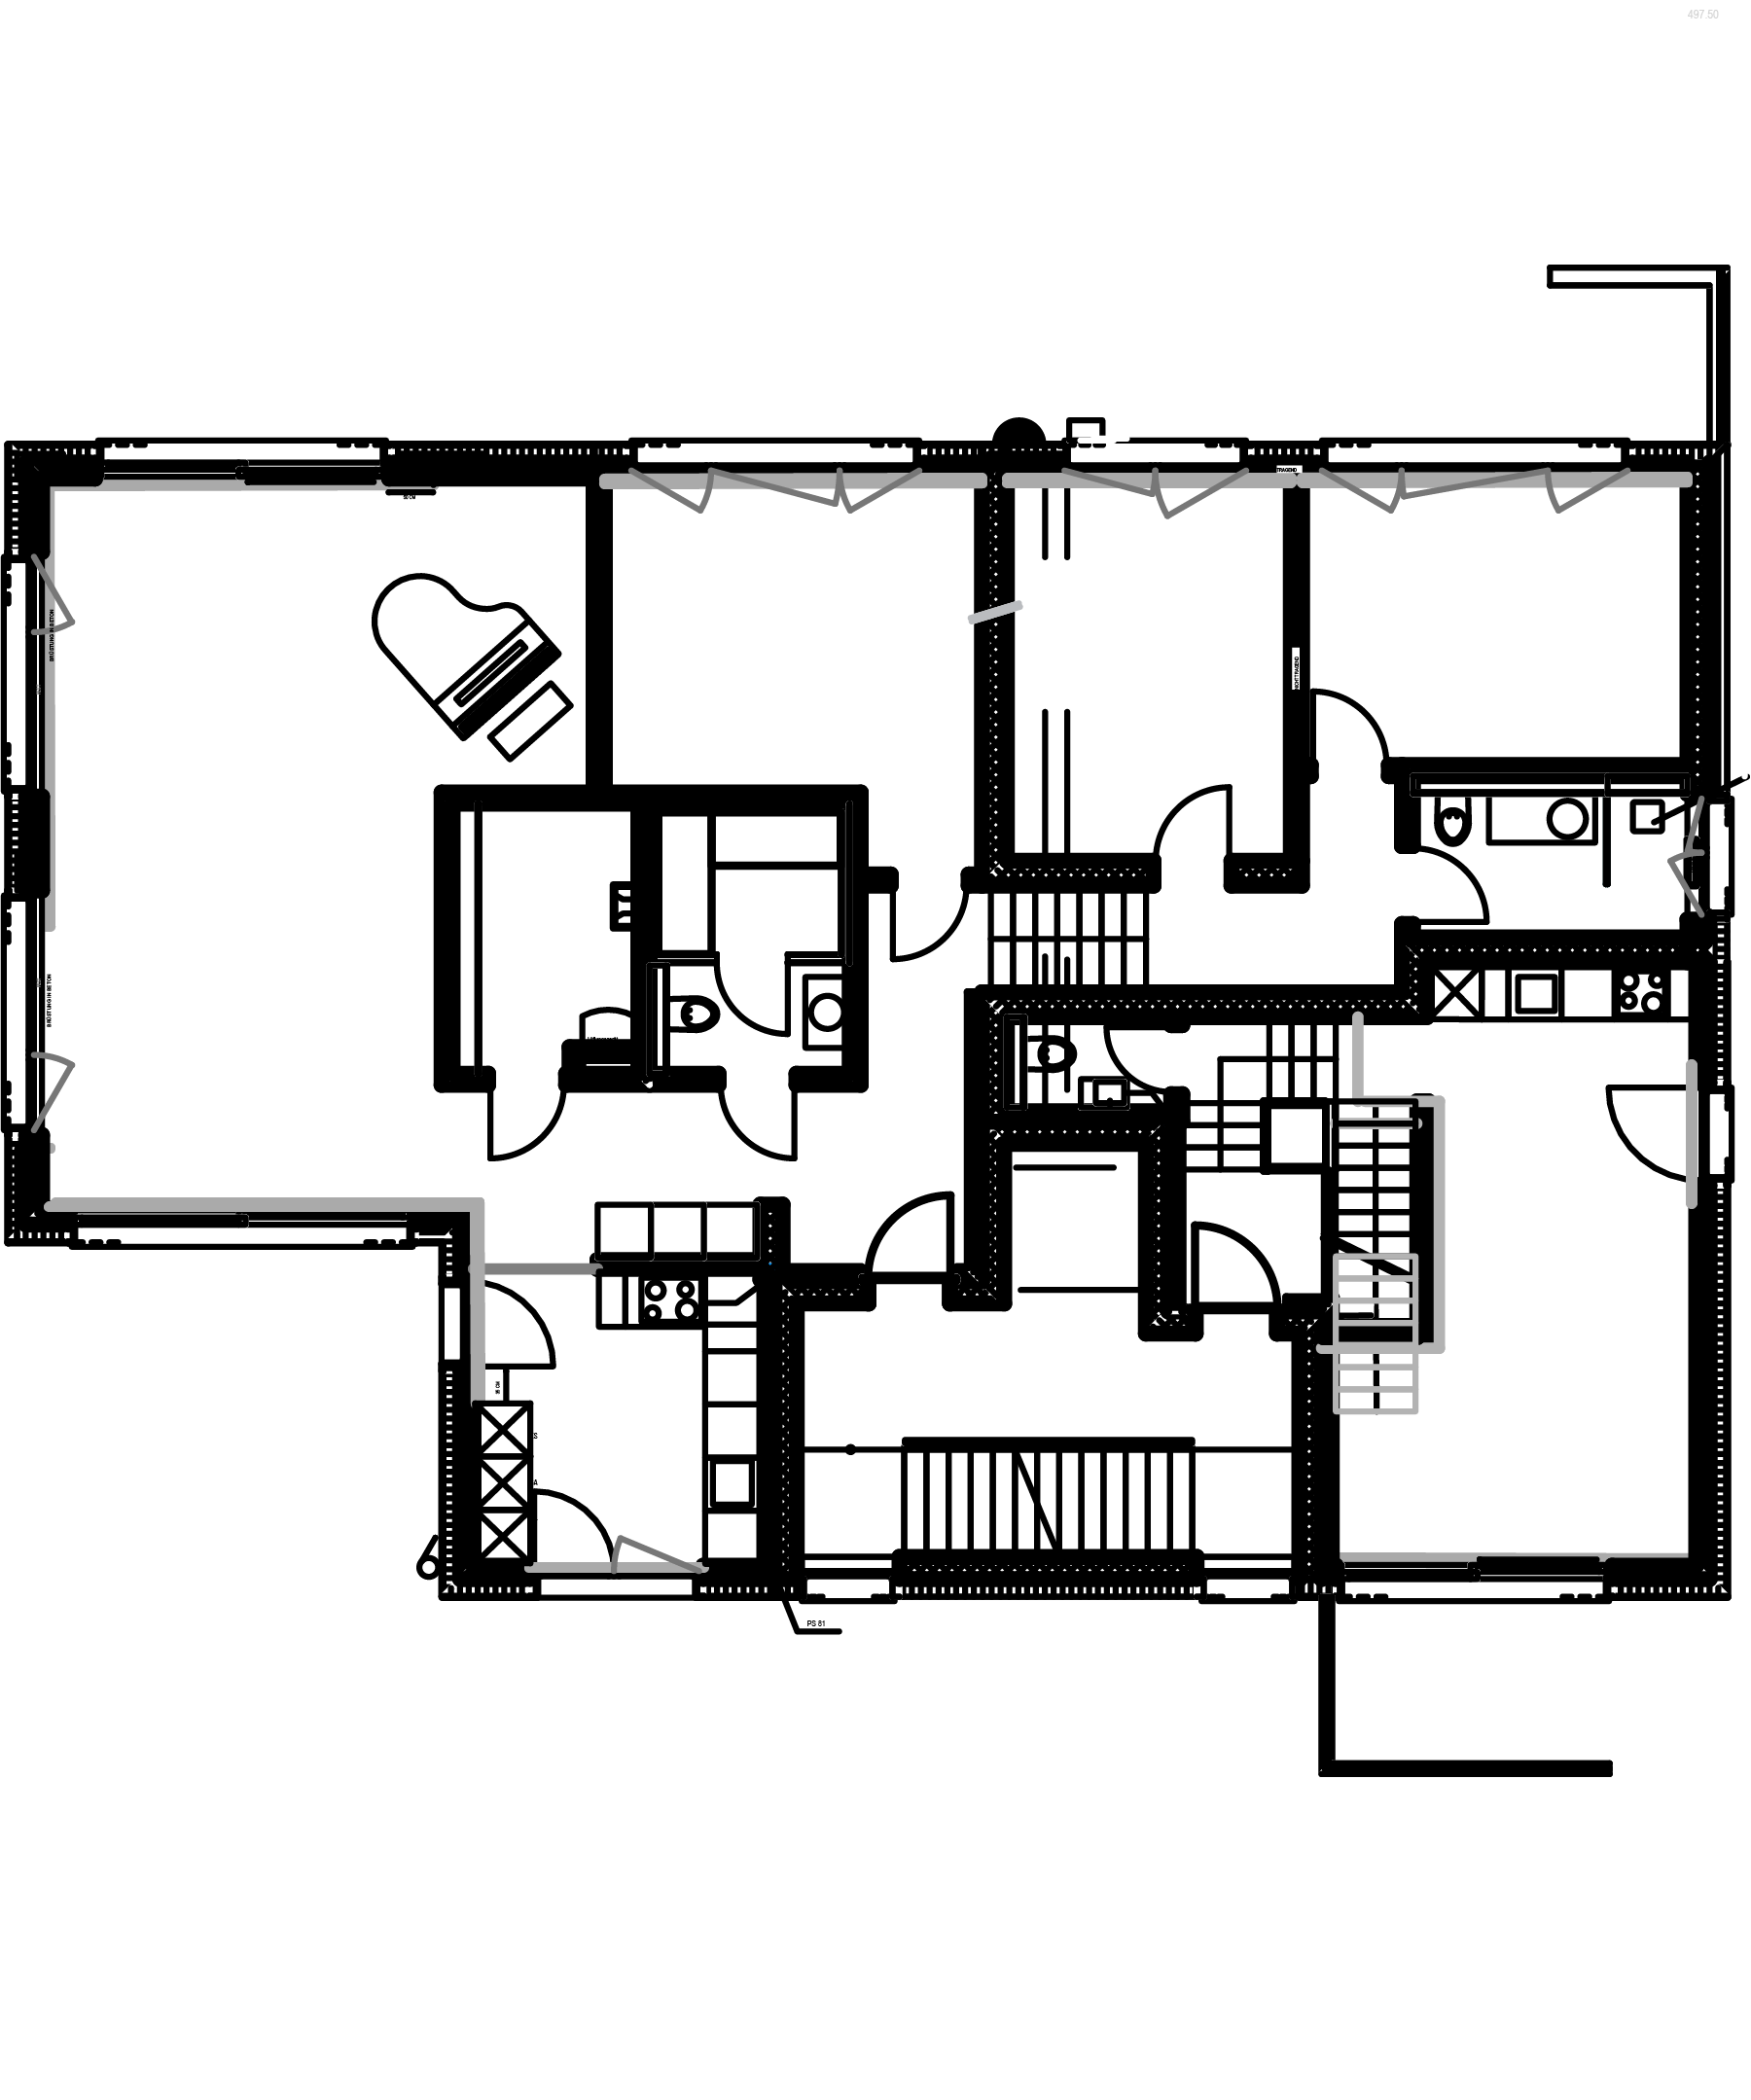
\includegraphics[width=0.5\textwidth]{A_N1_cleaned.png}\label{fig:A_N1_cleaned}}
	\hfill
	\subfloat[Image after noise removal.]{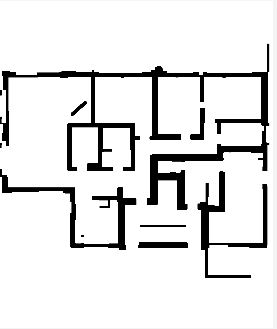
\includegraphics[width=0.4\textwidth]{morphtranscleaned.jpg}\label{fig:A_N1_cleaned_Morph}}
	\caption{Before and after of a cleaned floor plan with noise removal.}
\end{figure}

The figure~\ref{fig:A_N1} is one of the uncleaned testing images before any noise removal. It was cleaned up with an erosion/dilation size of 8. Figure~\ref{fig:A_N1_Morph} is the result of the noise removal. It is easily visible that most of what's left are walls. Due to the thin lines of the windows they get removed in the process. Those will be added later though, as they are an important part of the wall to surround the rooms.

The same was done to the cleaned up image. As a result of different image sizes, the noise removal was actually worse with the same parameters. This shows that each different image has very specific parameters for an optimal noise removal.

As this is not perfect due to the variety of possible objects on a plan, there is the option to delete either before or after with our built in editor. This is so that we can manually improve the quality of the outcome of noise removal.

As a result of the noise removal, we get an image with very basic information about where the walls are. This will be very important for our next step and other steps to come.


\subsubsection{Room detection}
To implement the room detection, the preprocessing had to be improved compared to the first workflow. What was needed is a proper creation of the foreground and background image. The foreground image contains all the centers of the room. Each center receiving its own color value to differentiate them from each other. The background image contains all the walls. Those are then combined into a single image and handed over to the watershed algorithm that then finds the rooms. The center of the rooms are found with a combination of a distance transformation~\ref{sub:DistanceTransformation}, a geodesic dilation~\ref{sub:GeodesicDilation} and a contour finding~\ref{sub:FindContours}. All of those are described in the following paragraphs.

\paragraph{Distance transformation}
\label{sub:DistanceTransformation}
The distance transformation is used to find the centers of the rooms as explained in section~\ref{subsubsec:Distance transformation}. As its base it needs a cleaned up image of all the walls. It is a result of the noise removal we discussed in the previous section. To find the actual area of the of the room there is further processing with a geodesic dilation (Section~\ref{subsubsec:GeodesicDilation}) needed.

The distance transformation gives us an image that represents the distance from the walls (lines in black) as a gradient of grey values going from dark (close to the wall) to bright (farther away). This means that there will be a center in each room that is very bright and has color values close to white.

\begin{figure}[H]
	\centering
	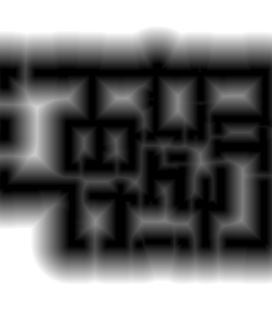
\includegraphics[width=0.8\textwidth]{dist_transform.jpg}
	\caption{Example distance transformation of a architectural floor plan.}
	\label{fig:dist_transform}
\end{figure}

To find the centers, there had to be an additional method that provides us with a specific information where these center areas are.
\todo{Discuss specific parameters for each image in parameter finding}

\paragraph{Geodesic dilation}
\label{sub:GeodesicDilation}
The algorithm to locate the centers after having done the distance transformation is the geodesic dilation~\ref{subsubsec:GeodesicDilation}. The purpose of this algorithm is to find the brightest points in an image and create a marker image. This marker image is a binary image that has all the bright points represented with white color and all other with black color. Based upon the assumption that the distance transformation marked points brighter the further away they are from walls, all room centers consist of bright pixels. Therefore the marker image contains all the room centers. Additionally though, since the plan usually has open space outside the bounding wall, it finds room centers outside of the house as well. The idea was that to close the outside walls and then delete all rooms that are connected to the border of the picture. There is an implementation of this algorithm in workflow 3~\ref{sub:WallClosing}. An implementation of how we tried to avoid this problem is described in the next paragraph about finding contours.

\begin{figure}[H]
	\centering
	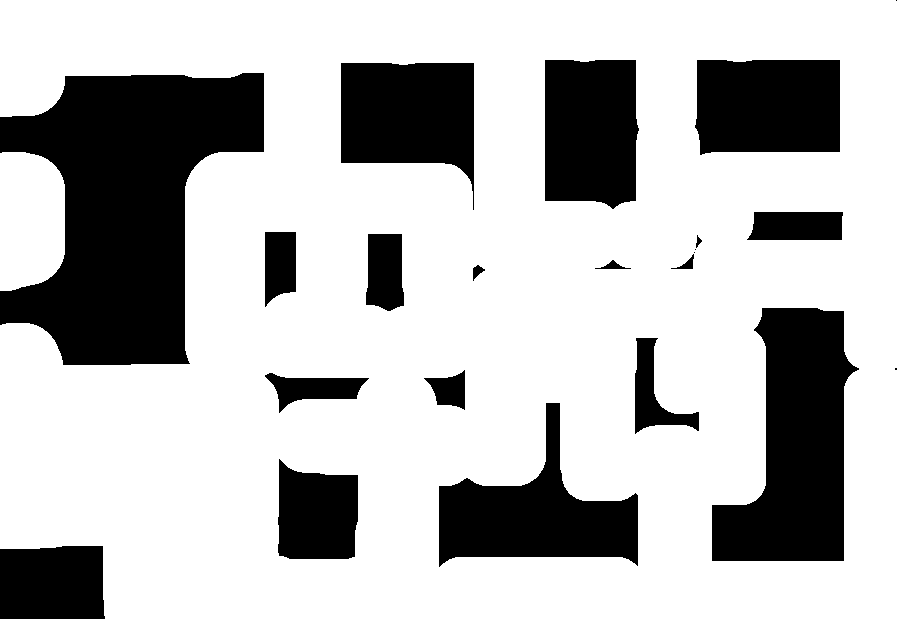
\includegraphics[width=0.8\textwidth]{MarkersGeodesicDilation}
	\caption{This image shows the markers (black areas) for the geodesic dilation of the floor plan AN1.}
	\label{fig:geodesicDilation}
\end{figure}

\paragraph{Find contours}
\label{sub:FindContours}
The find contours algorithm was used to find the centers found in the marker image and give each of those their own color value. This was done so the watershed algorithm automatically creates a border between rooms as soon as the different flooding zones from the algorithm meet each other. This process is further described in the next paragraph. What the find contours algorithm does on the marker image is, that it finds all the borders of the defined centers. With the implementation of findContours in OpenCv you can specify to also fill the found borders with a specified color value. Therefore, each marker found got a new color value. As it is a grayscale image, a base value of 200 was defined and for each new room found we increased that color for that room by one. This gives the option to detect up to around 50 rooms.

\begin{figure}[H]
	\centering
	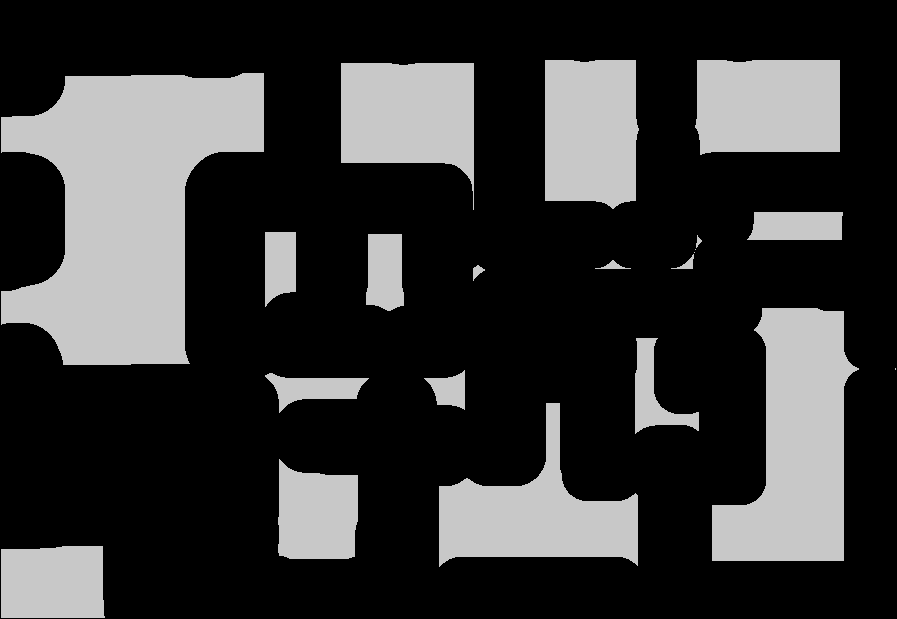
\includegraphics[width=0.8\textwidth]{findContourForeground}
	\caption{This image shows the different marker centers colored in pixel values around 200 and higher on the plan AN1.}
	\label{fig:findContour}
\end{figure}

An additional idea that was tried was to ignore rooms found that had any connection to the border of the image. The findContours algorithm finds a hierarchy on what contour contains other contours. We therefore tried to use the heuristic that the out-most contour that contains all other contours is the contour that contains all "room-centers" that are outside of the house. Therefore this contour could be ignored. As you can see on the image \ref{fig:geodesicDilation}, this heuristic does not work very well as there are too many conditions that can make it fail. One problem was that windows weren't closed and actual room centers existed that connected to the wall itself and therefore were not an inner contour. Additionally, there are sometimes inner contours that are not part of the house itself. As a result of those experiments we came up with a solution that is described in workflow three as wall closing~\ref{sub:WallClosing}.

 
\paragraph{Watershed}
\label{subsubsub:watershed}

The watershed is the core of our room search algorithm. Its purpose is to fill  the unknown areas that are provided in a foreground/background image from previous images. It needs extremely good preprocessing. If it has any previous errors, the resulting rooms will not make sense.

We use the watershed and its ability to find connected rooms with a simple method. It is a simple algorithm that has low computational cost. This and the fact that it was already implemented in openCV, made us use this algorithm.

The algorithm uses a simple image of all the walls as an image to compare to the foreground/background image. This image has been modified with the door recognition algorithm to close all doors within that picture. This is important so rooms are separated when running the watershed algorithm. Additionally, we tried to do a window recognition to close the outside walls. As explained in section \ref{sub:WallClosing}, this did not work out as planned. What we instead used is explained in the second part of section \ref{sub:WallClosing}. With this method we are able to separate all rooms within a building that has no windows on the inside. Any building that has a courtyard will fail with this method. Our goal was to find a solution that can also deal with this. But due to limited time and no reasonable alternative, we chose to go with that.

The background/foreground image is split up in three different zones. The zone with pixel color values of 0 represent the part of the image that are unknown. All pixels with color value 128 represent the walls. As for the rooms, we chose to mark all center with value 200. The image used for comparison has the same areas with walls as the BG-image. This means that the area for the wall will not expand with the watershed. The only exception is the area where doors or windows were closed. This is based on the assumption that the wall has the same pixel color and the inside of the room has a vastly brighter color.
The bright centers of the room inside the BG-image will expand into the unknown areas close to the walls and fill up the rooms. This will result in an image with several enclosed rooms all having the same pixel color. This will be processed with a modified connected component algorithm to find all the edges or the room.

We ran into several problems during the implementation of this algorithm. The most common problem is that not all doors were found. Furthermore, not all rooms have doors to separate them. There are also rooms that are separated with just an open space. There are also objects like cabinets that were drawn with thick lines and were identified as a part of the room. This is easily recognizable as a human but can not be differentiated with the algorithms used.

As a solution to the fact that not all the doors are found, there is the option to close doors by hand with the editor. This is the simplest solution that always guarantees success. We also tried to improve door detection with better samples and bigger sample size. This can be found in the section \ref{sec:ResultsCascade}.
To erase object from the image we initially planned to do an object detection. There was time to do some additional object detection other than just door and window. The cascade files can be found in the code. But there are too many different objects only within those few plans to catch them all. To implement object detection for further objects and erase those objects is a next step for this project. For now the user has to erase all object that do not get caught by noise removal by hand.


\subsection{Workflow 3}
\label{sub:workflow3}
With all the gained experience in workflow one (Section~\ref{sub:workflow1}) and workflow two (Section~\ref{sub:workflow2}), we started to implement workflow three. This workflow improves the room detection with the use of object detection, to fill gaps caused by the morphological transformation (Section~\ref{sub:MorphologicalTransformation}).

\begin{figure}[H]
	\centering
	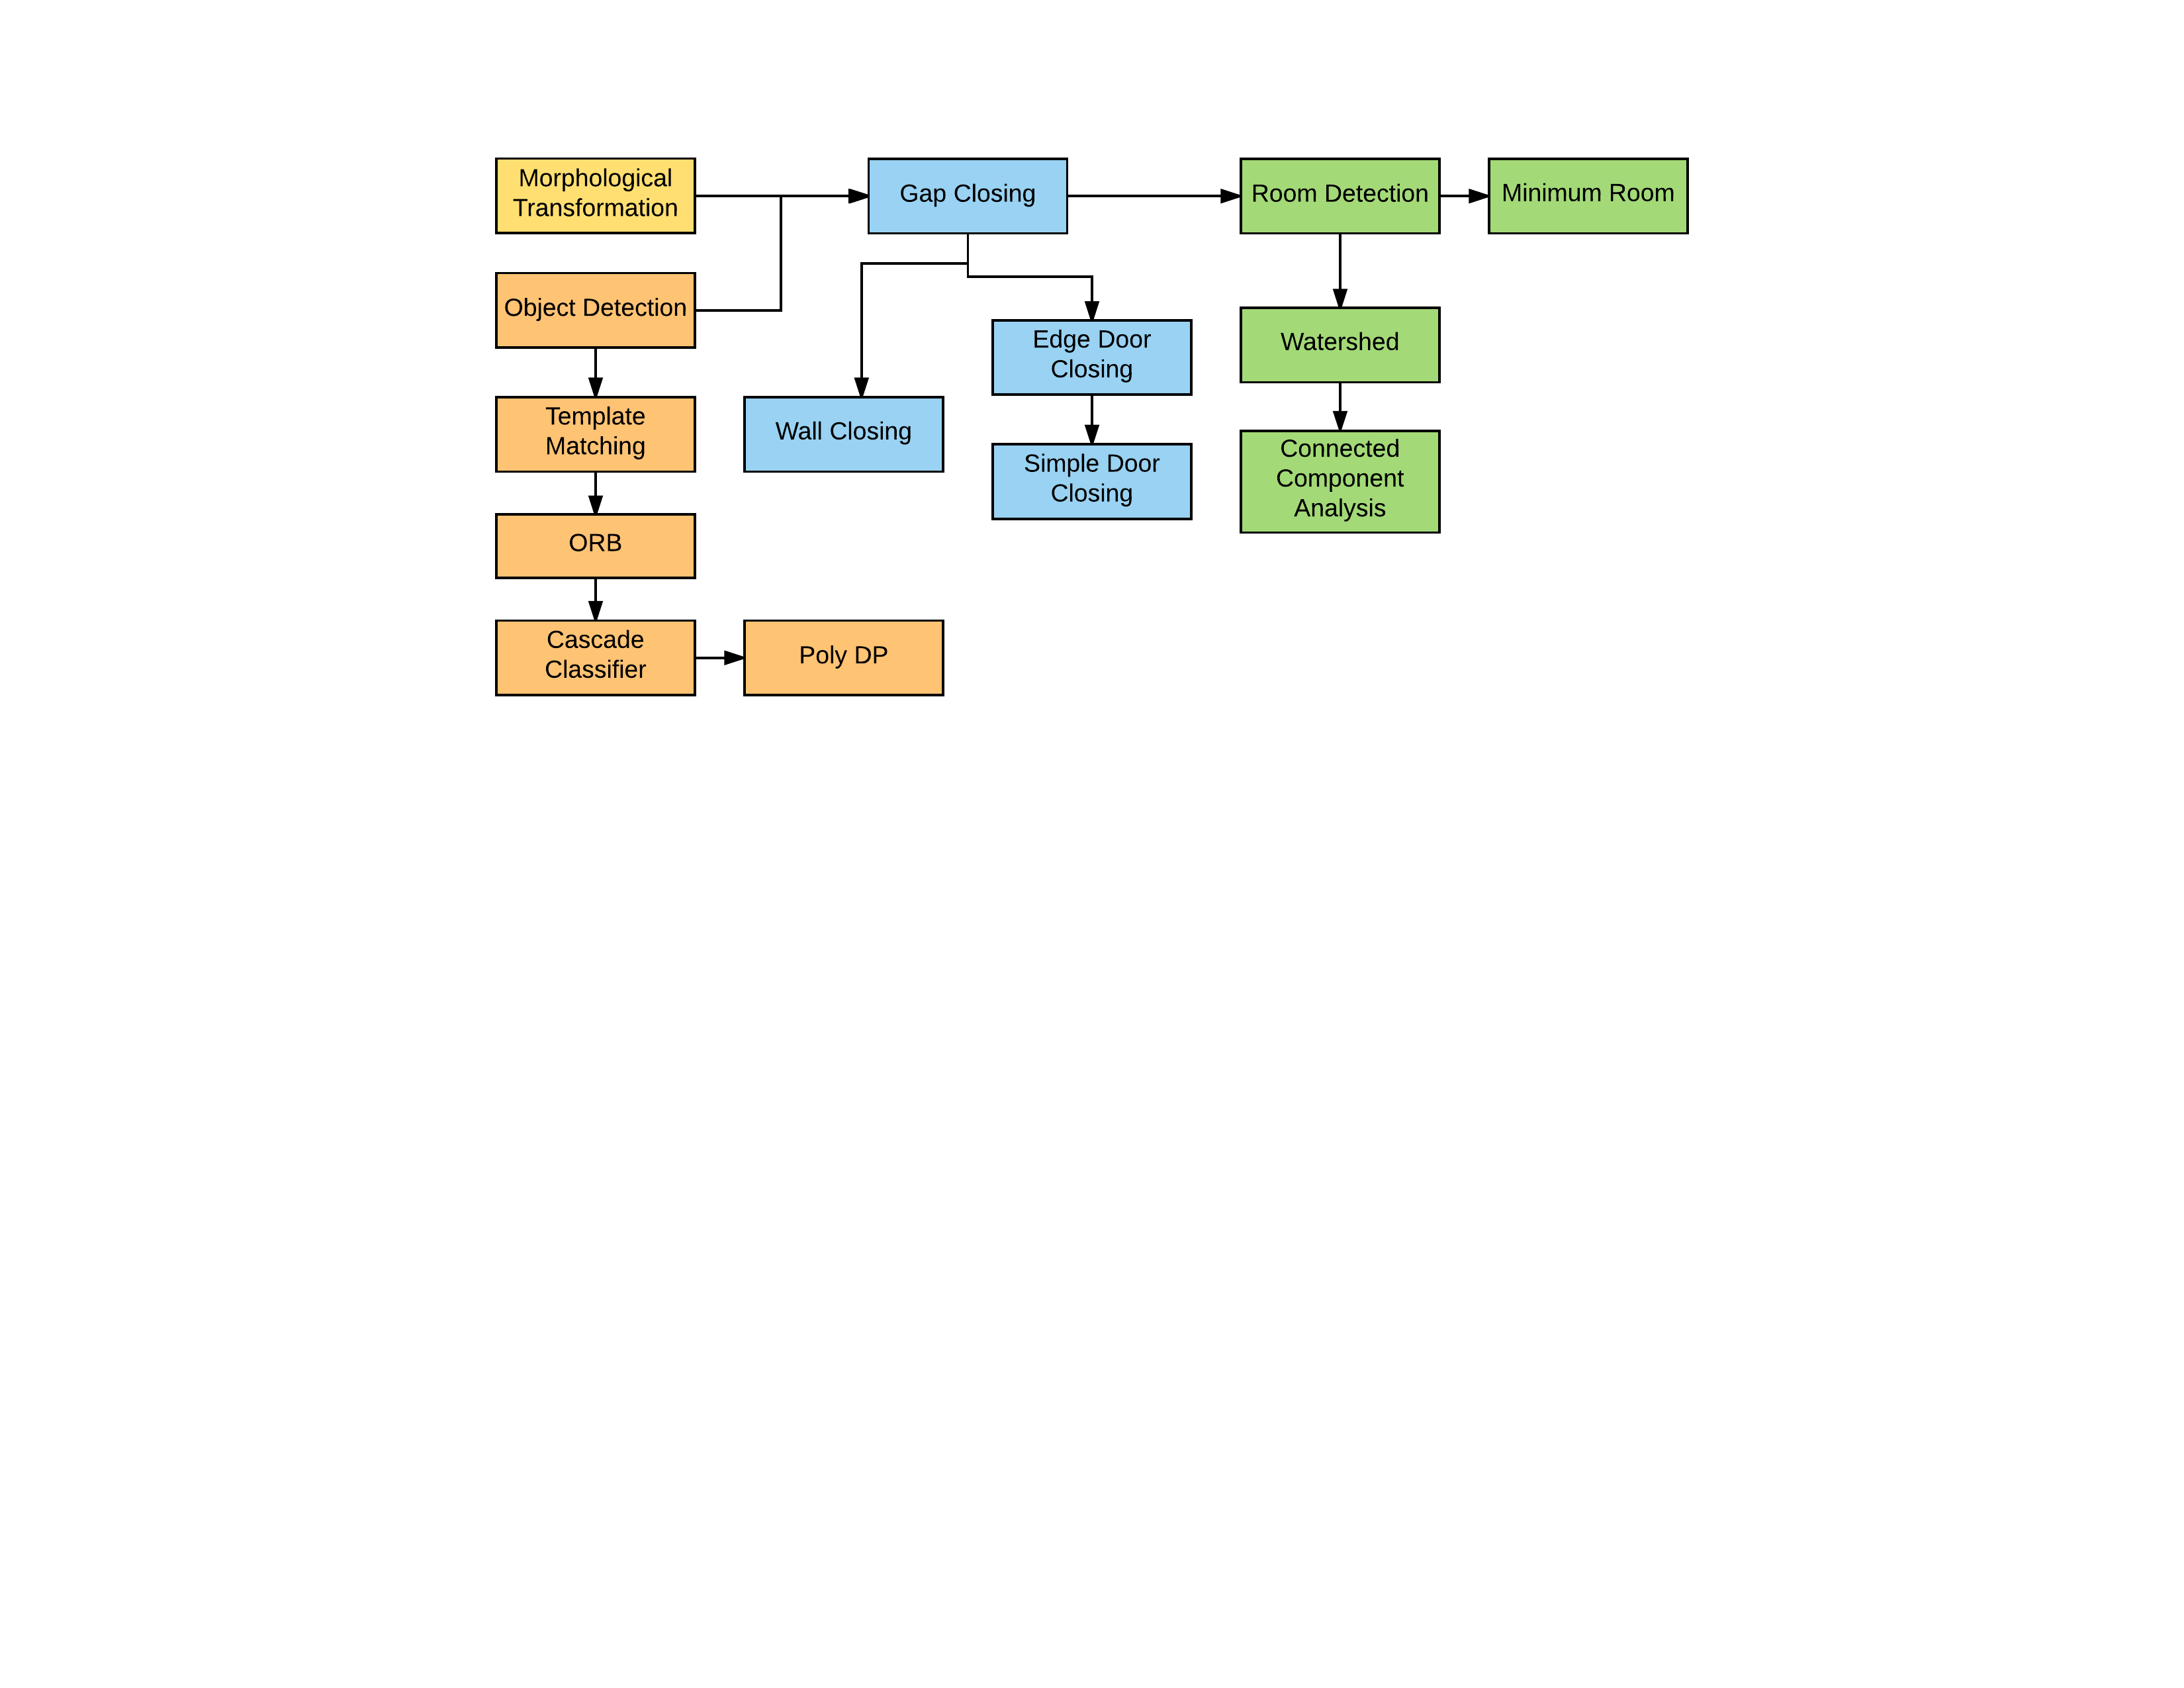
\includegraphics[width=1.0\textwidth]{Workflow3Flowchart}
	\caption{Workflow 3 flowchart.}
	\label{fig:Workflow3Flowchart}
\end{figure}

As shown on figure~\ref{fig:Workflow3Flowchart}, the morphological transformation and object detection step can be run in parallel. Because the user interface needs the assistance of the user, we decided to first run the object detection and then run the morphological transformation.

\subsubsection{Noise removal}
\label{sub:NoiseRemoval}
Noise removal has not been changed from the previous workflow. Morphological transformation is still used in this workflow, to detect the inner and outer walls of the building and to remove unwanted noise from the image like furniture or architectural markings.

For more information about the noise removal, have a look at section~\ref{sub:MorphologicalTransformation}.

\subsubsection{Object detection}
\label{sub:ObjectDetection}
One of the major problems of workflow two (Section~\ref{sub:workflow2}) is, that the morphological transformation erases too many elements from the floor plan. The doors and windows are also removed, but they are needed to separate the individual rooms.

Object detection was contemplated from the beginning of the project, to detect furnishings and other parts of a room, which define the room zones (Section~\ref{sub:RoomZones}). So the idea was to use it to detect doors and windows, and close the gaps between the walls. This would solve the problem of workflow two.

The basic problem was to find an algorithm that can detect objects that vary in their details, regardless of their rotation and size. This is important due to the fact that there is no standard for objects in architectural floor plans that are used by a wide audience of architects. The decision to go with a machine learning approach and not an algorithm that works with heuristics, is because we wanted to be able to process a broad variety of floor plans. Regardless whether they show a small house with just basic features, or a big plan with a lot of details and special objects.

In the following sections, we will take a look at different object detection approaches and how well they performed in detecting doors. The performance for each algorithm will be measured with the F1 score (Section~\ref{sub:F1Score}).

\begin{table}[H]
\centering
\caption{Floor plans with total count of rooms and doors.}
\label{tbl:FloorPlanData}
\begin{tabular}{@{}lll@{}}
\toprule
Name          & Rooms & Doors \\ \midrule
50er\_eg      & 21    & 26    \\
A\_N1         & 9     & 13    \\
A\_1OG        & 50    & 75    \\
Grundriss\_OG & 4     & 2     \\
H\_OG01       & 12    & 19    \\ \bottomrule
\end{tabular}
\end{table}

Table~\ref{tbl:FloorPlanData} shows each test floor plan, with its number of rooms and doors. The data has been raised by hand and does not include doors, windows or closets. This data will be used to calculate the metrics of each object detection algorithm.

To test the algorithms, we decided to just use three of the five experiment images (\textit{50er\_eg}, \textit{A\_N1}, \textit{A\_1OG}). This is due to the fact, that we have to run the test on the original version and the cleaned version of the image. These three images represent the average floor plans, that will be processed by this software.

\paragraph{Template matching}
\label{sub:ImpTemplateMatching}

Template matching is a very simple matching method, which can be used to find one or multiple occurrences of a template $T$ in an image $I$. For a better understanding of the algorithm, have a look at section~\ref{sub:TemplateMatching}.

First of all, we have to define the template $T$ (Figure~\ref{fig:DoorTemplate}), which in our case is a door of the floor plan \textit{AN\_1}.

\begin{figure}[H]
	\centering
	
\includegraphics[width=0.2\textwidth]{door_template}
	\caption{Template $T$.}
	\label{fig:DoorTemplate}
\end{figure}

If we run the template matching algorithm on an image, it returns a correlation matrix of the input image. Brighter spots indicate that the area correlates better. Now to retrieve the best correlated areas, we threshold the image with a threshold value of \textit{250}, to only get the best correlation locations. These bright spots are then analysed with the connected component analysis (Section~\ref{sub:ConnectedComponentAnalysis}), to count the amount.

\begin{figure}[H]
	\centering
	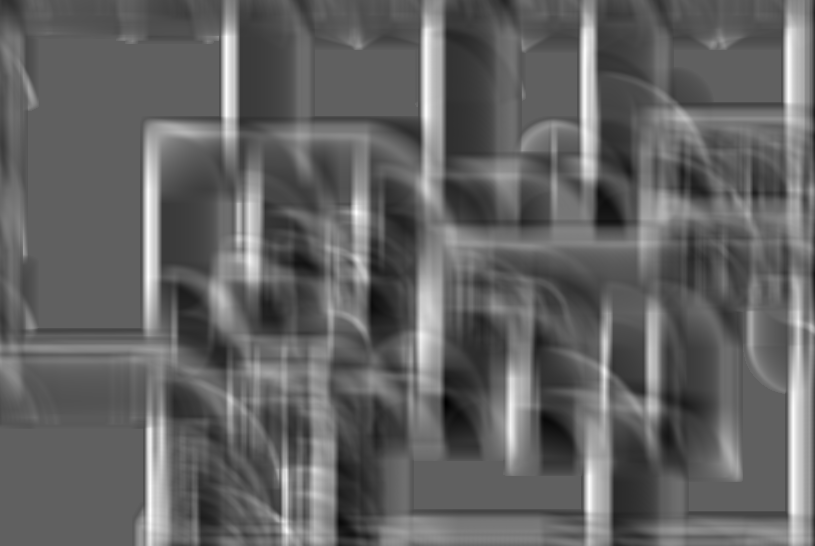
\includegraphics[width=0.8\textwidth]{TMAN1Correlation}
	\caption{Correlation matrix of \textit{A\_N1\_C}.}
	\label{fig:TMAN1Correlation}
\end{figure}

As shown on figure~\ref{fig:TMAN1Correlation}, the template correlates with a lot of objects in the image, like the walls. Instead of doors that will be recognised, the algorithm returns a lot of false positives and only one true positive.

\begin{figure}[H]
	\centering
	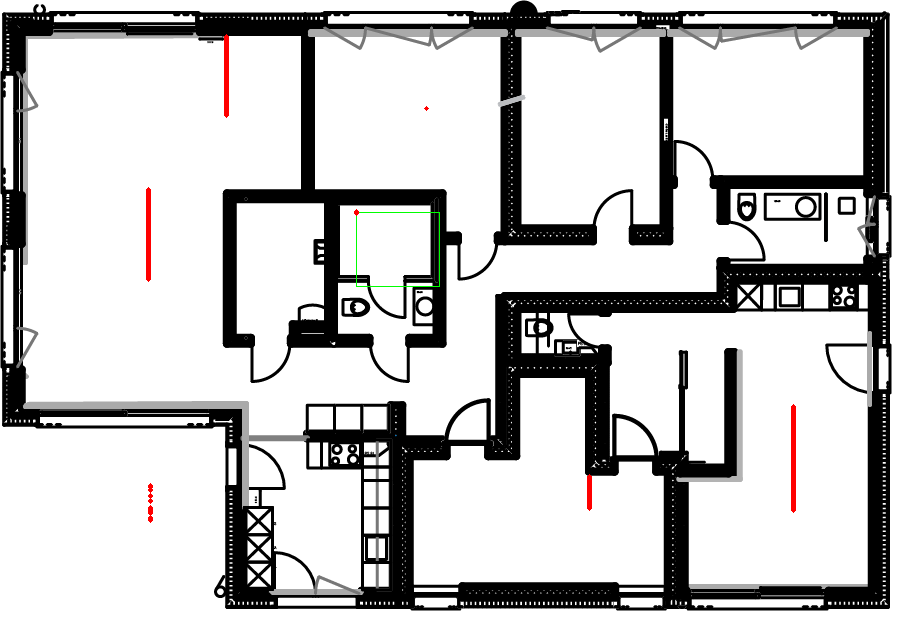
\includegraphics[width=0.8\textwidth]{TMAN1Result}
	\caption{Image \textit{A\_N1\_C} with detected doors.}
	\label{fig:TMAN1Result}
\end{figure}

This over-correlation can also be seen in figure~\ref{fig:TMAN1Result}, which shows the result of the component analysis. The red areas are the marked bright spots of the correlation matrix. Only one door in the middle of the plan is marked close to its location. This door is counted as true positive, even if the location does not perfectly fit.

\begin{figure}[H]
	\centering
	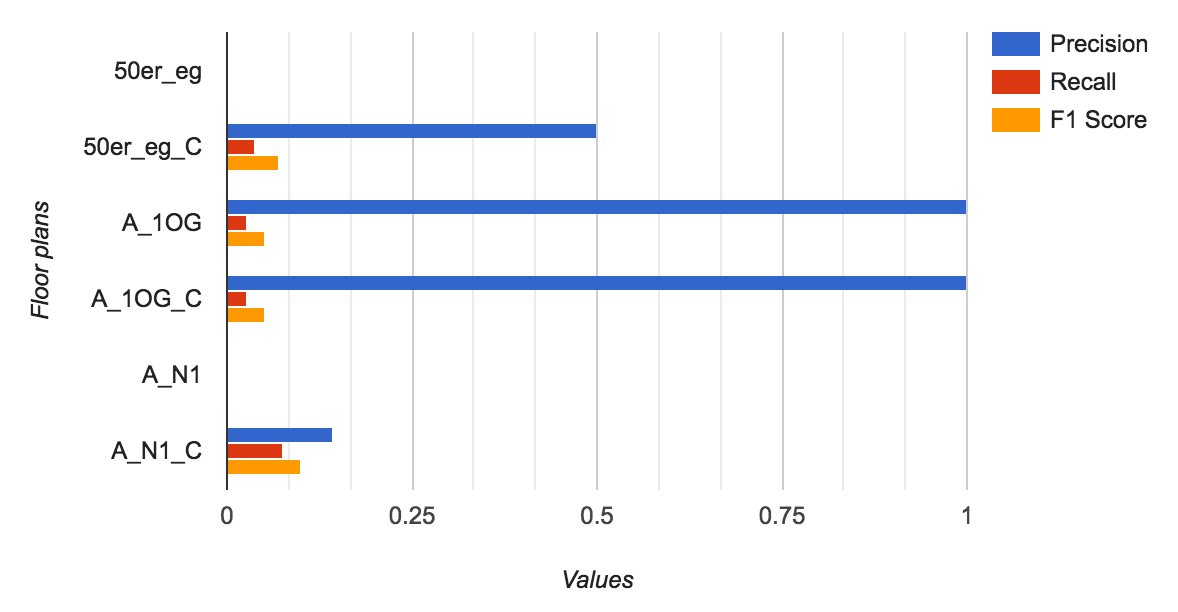
\includegraphics[width=1.0\textwidth]{TMResultDiagram}
	\caption{Results of the template matching experiment.}
	\label{fig:TMResultDiagram}
\end{figure}

This behaviour is also recognisable in the result graph (Figure~\ref{fig:TMResultDiagram}). The precision is very high, if something was detected. This is attributable to the fact, that very few positives have been detected. Recall instead is very low, because of the same reason. If no positives are recognised, whether \textit{true} or \textit{false}, the recall is very low. This is also reflected by the F1 score, which is nearby zero.

Interesting to mention is, that over all floor plans, the cleaned version (\textit{NAME\_C}) is better for the template matching, than the original image. But even the results of the clean versions are very poor.

We think that this bad result arose, because the template matching algorithm is not scale or rotation invariant. This leads to very few true positives. On the other hand, the correlation matrix shows, that the doors correlated with every straight wall on the plan. This could be a problem of the very common shape of doors.

\paragraph{Oriented FAST and Rotated BRIEF (ORB) OpenCV}
\label{sub:ImpORB}

As you see in the results of the template matching method (Section~\ref{sub:ImpTemplateMatching}), the scale and rotation variance of the algorithm delivers very bad results. The idea with ORB is to use an algorithm for object detection, which is rotation and scale invariant.

We use the algorithm implemented in \textit{OpenCV 3.1}. ORB also takes a template image $T$ and tries to find the objects in the image $I$. But ORB tries to find scale and rotation invariant features on the template image $T$. These feature are used to run the detection (Section~\ref{sub:ORBAlgorithm}). 

For our tests, the same template $T$ is used, as for template matching (Figure~\ref{fig:DoorTemplate}).

After implementing the algorithm, we recognized, that it was not able to detect any objects on the images. A visualisation of the features of our template image $T$ showed, that zero features have been detected in our image. Our investigations lead us to the conclusion, that the \textit{nFeatures} parameter of the ORB algorithm, was to low.

We tried to increase this feature count, but then realised, that it is not possible to set parameters for detectors in OpenCV 3.1. The problem is that the method, to read and write algorithm parameters, is implemented in the Java wrapper, but is missing in the C++ implementation (see \citep{orb}).

\paragraph{Oriented FAST and Rotated BRIEF (ORB) JavaCV}
\label{sub:ImpORBJVCV}
We then tried to use JavaCV to be able to access all parameters. The difference to OpenCV's method call is that each parameter can be specified. The problem with that approach was that the matrices used for JavaCV and OpenCV are different. Therefore, we had to copy the whole image, process it and then copy it back into the old matrix. To do this efficiently we had to use a buffer, or do it manually by hand. Both of those options took a lot of time as well as lot of memory and the buffer usually ran out of memory with larger images. At the same time, we had a different approach with the Cascade classifier in the pipeline, which looked a lot more promising. Therefore, this idea was put on hold and as the cascade classifier turned out very promising, it was never actually completely implemented.

\subsubsection{Cascade classification}
\label{sub:ImpCascadeClassifier}
The following section describes the cascade classifier algorithm to detect doors and other objects on the floor plan. After a short introduction, we will discuss the results and improvements of the different iterations of the algorithm training.

The cascade classifier is used for object recognition of doors, windows and other objects that are important for the room detection and zone identification. This algorithm is a machine learning algorithm that has to be trained with positive and negative images. The resulting learned parameters are saved in an XML file (Section~\ref{sub:CascadeTraining}). In the next section, the implementation process is described as well as all the experiences we made during this project.

The algorithm itself is trained with positive and negative images. It took multiple iterations to get to the trained classifier, we now use in the project. Each iteration differs by the parameters we have set during the training stage and the images we trained with.

\paragraph{Iteration 1 (CC\_T1)}
\label{sub:CCT1}
The first iteration of the training was to test out the capabilities of the cascade classifier. The results were not satisfying, but at least we were able to recognise something. We used a window size of \textit{32x24} and about \textit{20} positives samples and \textit{5} negative images. The positive images were a mix between floor plans of the customer and floor plans found on the internet. Negative images were original floor plans, where the object to train was removed.

\begin{figure}[H]
	\centering
	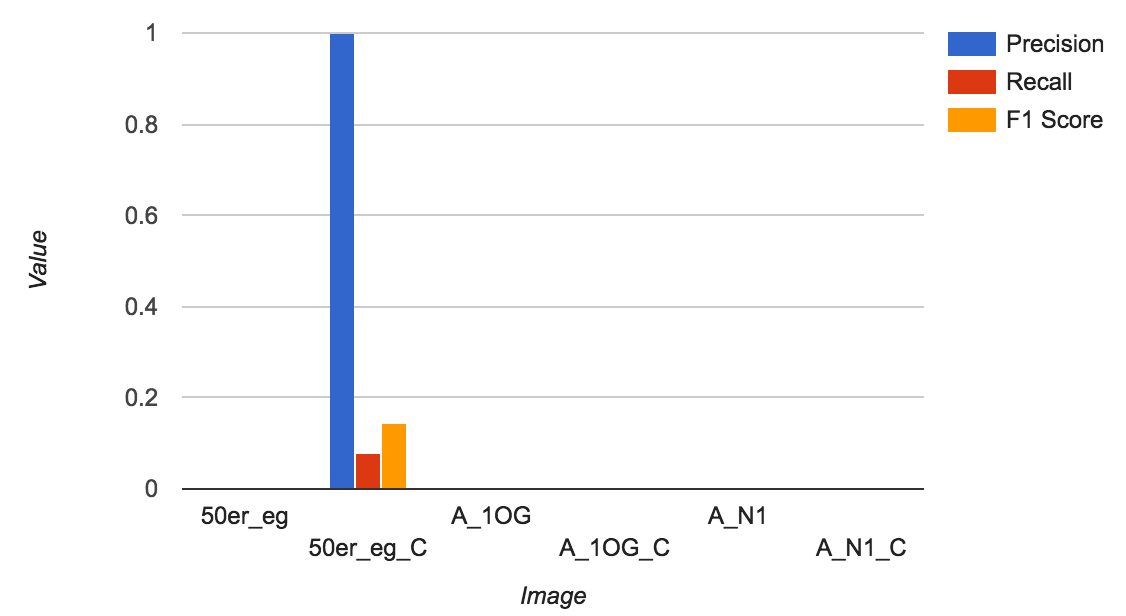
\includegraphics[width=1.0\textwidth]{CCT1Result}
	\caption{Results of the first cascade classification iteration.}
	\label{fig:CCT1Result}
\end{figure}

Figure~\ref{fig:CCT1Result} shows, that the trained classifier could not really find any doors on most of the floor plans. But if something was found, the precision is very high. This showed us that cascading classification is able to detect objects on a floor plan, but we needed to to detect more objects.

\paragraph{Iteration 2 (CC\_T2)}
\label{sub:CCT2}

Regarding iteration 1, we decided to increase the amount of positive samples to train more variations of doors. The second improvement was to lower the window size to \textit{20x20}. This lead to a better recognition of doors on floor plans with a low resolution. This is because the window size defines the lowest object size, which can be recognised by the cascade classifier.

\begin{figure}[H]
	\centering
	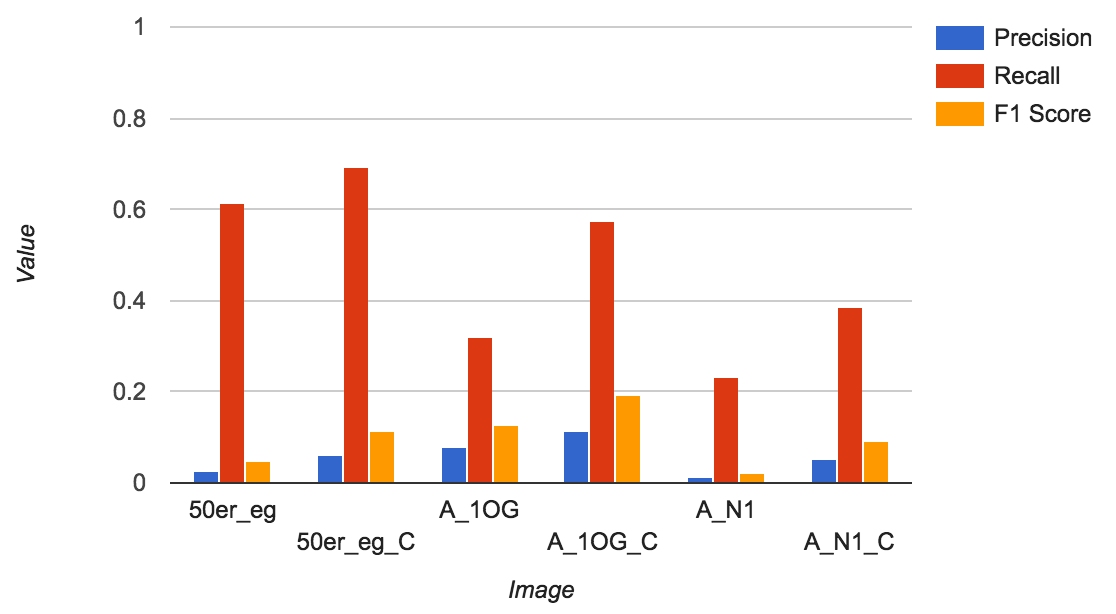
\includegraphics[width=1.0\textwidth]{CCT2Result}
	\caption{Results of the second cascade classification iteration.}
	\label{fig:CCT2Result}
\end{figure}

With this modifications, it was possible to detect much more objects on a plan then in iteration 1. The downside of this was, that the classifier was very inaccurate. There are very few true positives recognised, but a lot of false positives, which leads to a low precision (Figure~\ref{fig:CCT2Result}.

\begin{figure}[H]
	\centering
	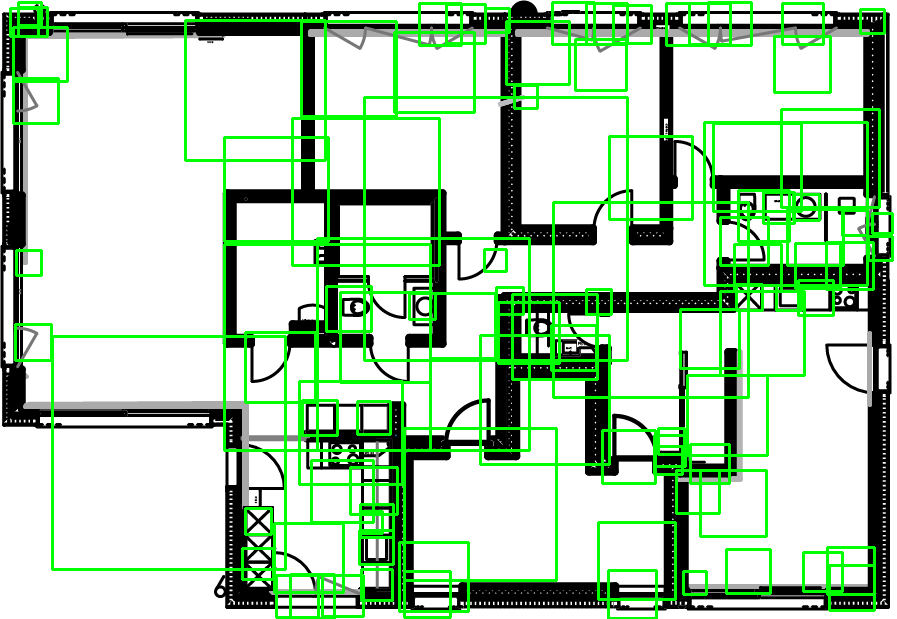
\includegraphics[width=1.0\textwidth]{CCT2ExampleAN1}
	\caption{Example of the second cascade classification iteration.}
	\label{fig:CCT2ExampleAN1}
\end{figure}

Figure~\ref{fig:CCT2ExampleAN1} shows an example of how the second iteration was performing. Nearly every element on the floor plan is detected as door. This lead us to the conclusion, that the door is trained with too few features, like the ORB method did (Section~\ref{sub:ImpORB}).

\paragraph{Iteration 3 (CC\_T3)}
\label{sub:CCT3}

To increase the features which can be detected on the positive samples, the decision was made to add a thickening to the trained floor plans. This thickening was also applied to the test images with the same parameters.

\begin{figure}[H]
	\centering
	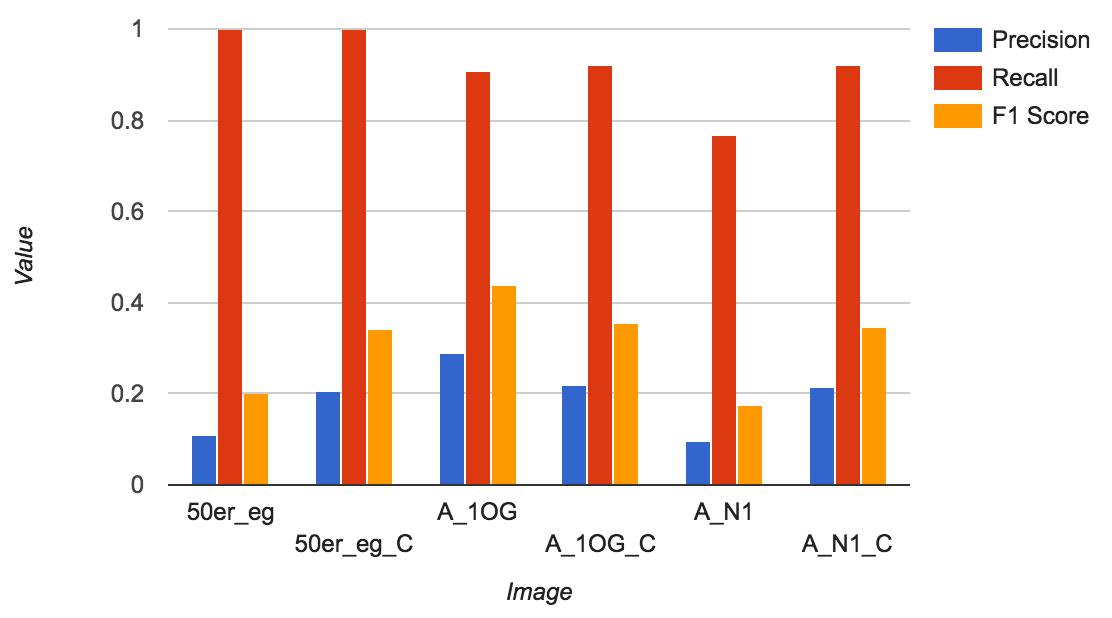
\includegraphics[width=1.0\textwidth]{CCT3Result}
	\caption{Results of the third cascade classification iteration.}
	\label{fig:CCT3Result}
\end{figure}

As seen on figure~\ref{fig:CCT3Result}, the precision slightly increased to iteration 2 (Figure~\ref{fig:CCT2Result}). This directly leads to a better F1-Score, because there were more true positives found in the images.

But the F1-Score is still very low, because a lot of the found images are not doors (false positive).

\paragraph{Iteration 3 with polygon matching (CC\_T3\_PolyDP)}
\label{sub:CCT3PolyDP}
\label{sub:PolyDP}

As improvement, we tried to use the cascade classification together with another method, which would classify the huge amount of positive images and filter out the false positives. The second method is called contour matching. It is a method to compare two shapes and get a value, which represents the difference between the two shapes.

\begin{figure}[h!]
	\centering
	\subfloat[Template door]{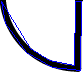
\includegraphics[width=0.3\textwidth]{PolyDPTemplate}\label{fig:PolyDPTemplate}}
	\hfill
	\subfloat[Matched door]{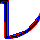
\includegraphics[width=0.3\textwidth]{PolyDPMatch163}\label{fig:PolyDPMatch163}}
	\hfill
	\subfloat[Matched door]{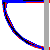
\includegraphics[width=0.3\textwidth]{PolyDPMatch41}\label{fig:PolyDPMatch41}}
	\caption{Shape matching template and matches.}
	\label{fig:ShapeDistanceMatching}
\end{figure}

To get the a template shape, we analyse the contours of the template image $T$ from the template matching method (Section~\ref{sub:TemplateMatching}). The largest contour on the template image (marked in blue on figure~\ref{fig:PolyDPTemplate}) is used as a template shape.

Now this shape detection is processed on every area, which the cascade classification has marked as positive. With the information of the largest contour, it is possible to calculate the distance to the template door. If both shapes have the exact same shape, the distance will be zero.

To filter out false positives, we have set a threshold, which only shows the areas, which match with a lower value than that of the threshold.

\begin{figure}[H]
	\centering
	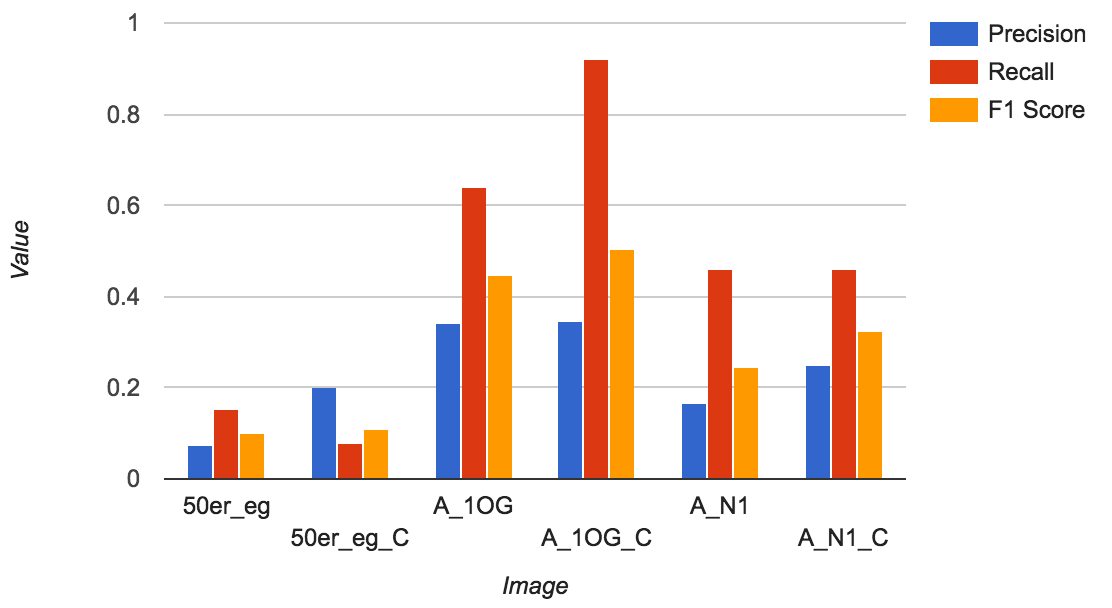
\includegraphics[width=1.0\textwidth]{CCT3PolyDPResult}
	\caption{Results of the third cascade classification experiment with shape matching.}
	\label{fig:CCT3PolyDPResult}
\end{figure}

To stack multiple detection methods behind each other was not as effective as we thought. As shown on figure~\ref{fig:CCT3PolyDPResult}, the F1-Score was on some images increased and on some decreased. This has to do with the template image $T$. It is very specific for one plan and if the doors do look a bit different on the plan, the contour will not match.

An advantage of this method is, that the amount of positive objects is decreased, because of the second filter method. But this also effects the recall on most of the images.

\paragraph{Iteration 4 (CC\_T4)}
\label{sub:CCT4}

After extensive research on how to improve the cascading classification method, we found an interesting blog post, which accurately describes how to get the best result from the training \citep{ball}. We realized, that the positive and negative sample ratio was not good for training small pictures like doors. In the previous iterations, we used a $2:1$ ratio, but it was recommended to use a $1:1$ ratio or higher.

We then decided to split up the large negative samples into very small pieces, to generate more negative images to train with. In the end we used about 600 positive samples and 600 negative samples.

\begin{figure}[H]
	\centering
	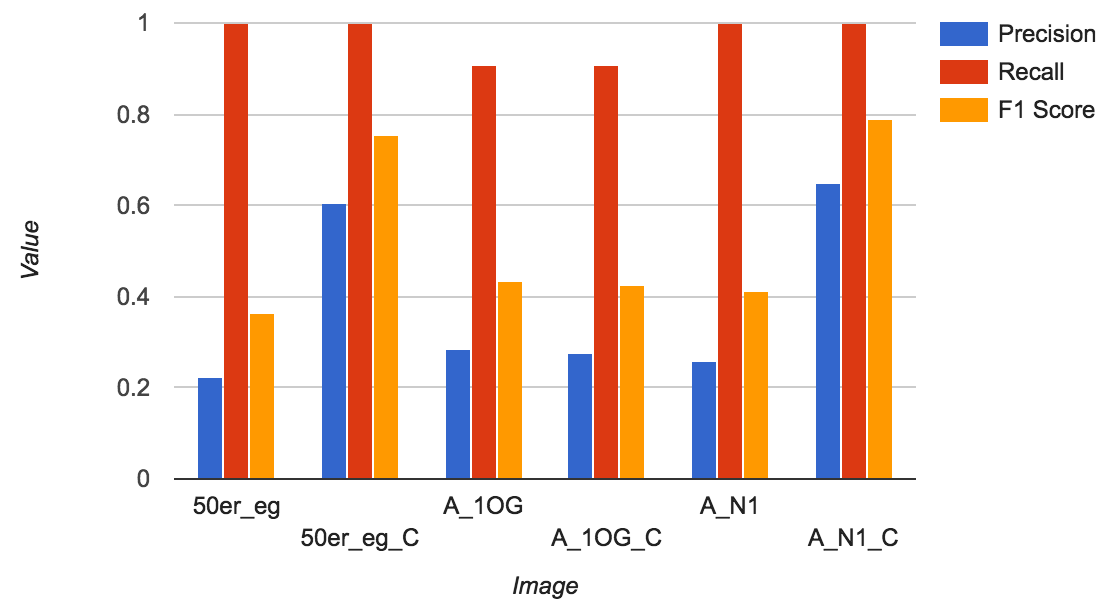
\includegraphics[width=1.0\textwidth]{CCT4Result}
	\caption{Results of the fourth cascade classification iteration.}
	\label{fig:CCT4Result}
\end{figure}

Actually, we used the same pictures like before, but the negative images have been cut into pieces. But this difference was a success as shown on figure~\ref{fig:CCT4Result}. The F1-Score is higher then ever before on every image. It was still not good enough, because there were some false positive detected, but not as much, as in previous iterations.

\paragraph{Iteration 5 (CC\_T5)}
\label{sub:CCT5}

In iteration five, we tried to improve the precision of the object detection, which was alright in iteration four (Section~\ref{sub:CCT4}), but still not good enough to use it in this project.

To increase the precision, we used even more negative samples to have a positive to negative sample ratio of $1:3$. As in iteration four, we used the big negative floor plans and cut them into very small pieces. In the end we used about 600 positive and 1500 negative images to train the classifier.

\begin{figure}[H]
	\centering
	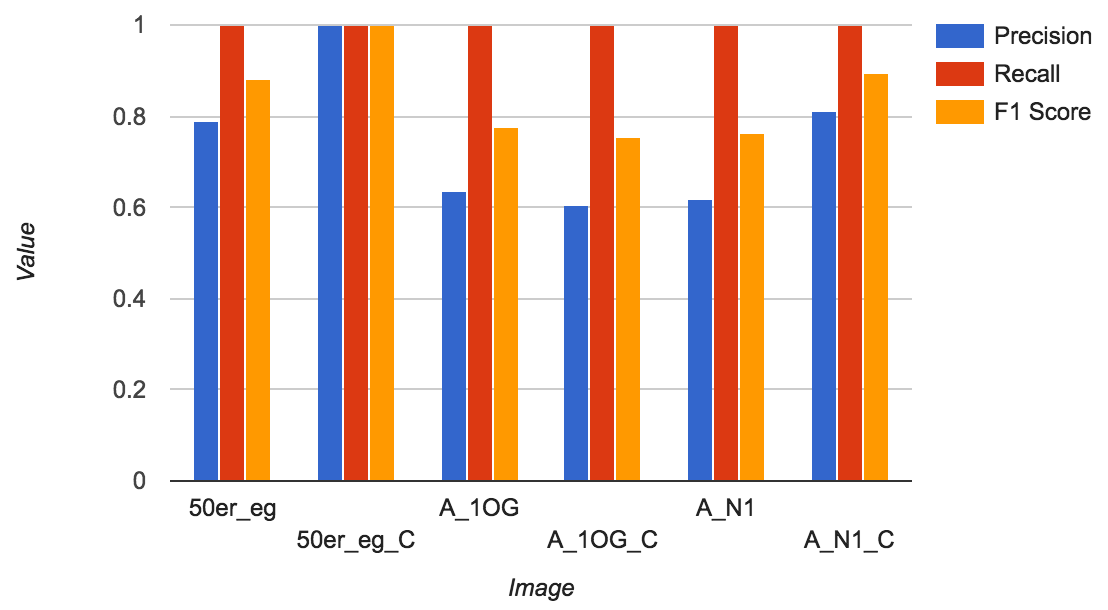
\includegraphics[width=1.0\textwidth]{CCT5Result}
	\caption{Results of the fifth cascade classification iteration.}
	\label{fig:CCT5Result}
\end{figure}

The results (Figure~\ref{fig:CCT5Result}) looked great. There were only very few false positives detected and, nearly all of the positives. The results seen in figure~\ref{fig:CCT5Result} originate from a test with fixed detection parameters. If we decrease the parameter \textit{minNeighbors}, the precision increases drastically. \textit{MinNeighbors} specifies how many neighbors each detected object should have, to retain in the result set.

\begin{figure}[H]
	\centering
	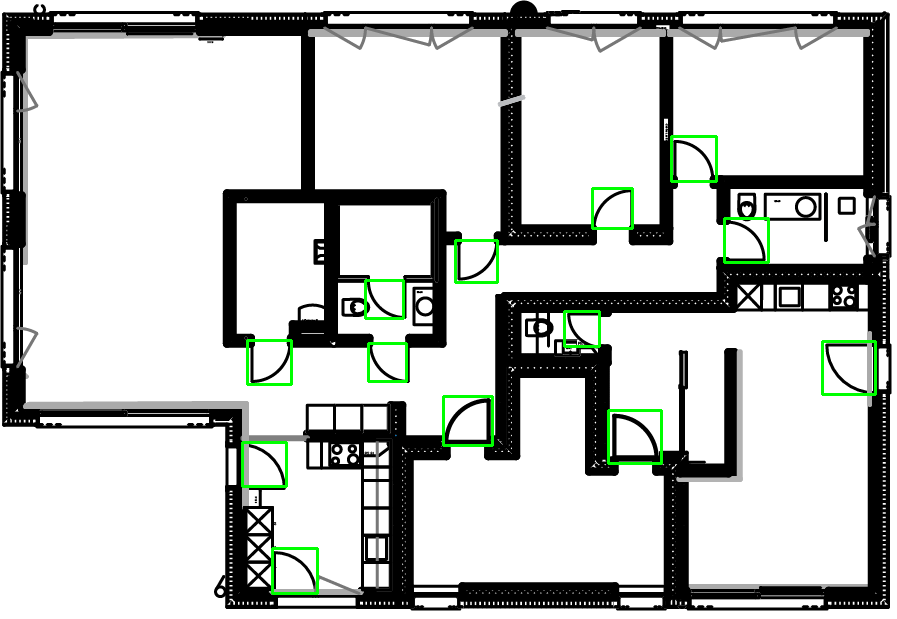
\includegraphics[width=1.0\textwidth]{CCT5ExampleAN1}
	\caption{Example of the fifth cascade classification iteration.}
	\label{fig:CCT5ExampleAN1}
\end{figure}

By default we use \textit{minNeighbors} with value $3.0$, but on some plans it is better to use a lower value. On the plan \textit{AN\_1} for example, it is better to use a value of 8.0 to get only the doors (Figure~\ref{fig:CCT5ExampleAN1}).

We currently use this training iteration for the door detection in the software. It is not perfect, but it is accurate enough to use and detect most of the doors.

\paragraph{Results}
\label{sec:ResultsCascade}
In this section, we will summarise the results of the cascading classification iterations and discuss the general improvements between each step.

\begin{figure}[H]
	\centering
	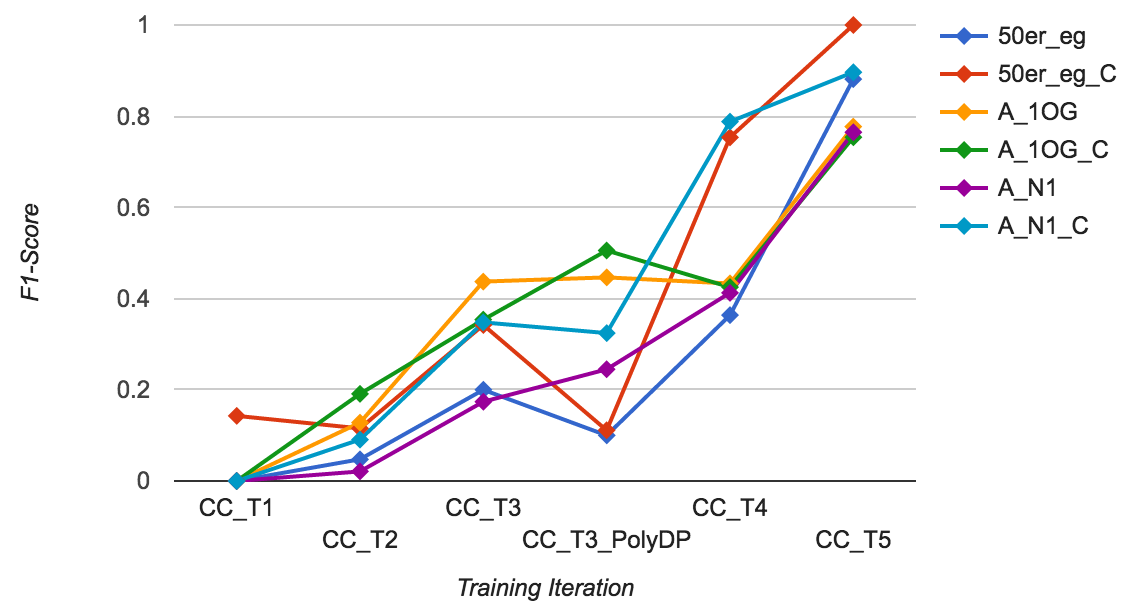
\includegraphics[width=1.0\textwidth]{CCF1ScoreGraph}
	\caption{F1-Score results of the floor plans.}
	\label{fig:CCF1ScoreGraph}
\end{figure}

Figure~\ref{fig:CCF1ScoreGraph} shows the F1-Score of each floor plan, over each training iteration. With more samples to train the classifier, the results increased over each training. Only the \textit{CC\_T3\_PolyDP} training was a retrogressive step, because the stacked filter system was too restrictive and rejected even true positives. In step \textit{CC\_T5}, all tested floor plans achieved an accuracy (F1-Score) over 75 percent, which was enough to use it in the gap closing algorithms (Section~\ref{sub:GapClosing}).

Another interesting graphic is the comparison between the performance of the original and cleaned floor plans. Figure~\ref{fig:CCF1ScoreGraphOCAverage} shows the averaged F1-Score of the original and cleaned floor plans, over each iteration. The cleaned floor plans always perform better then the original ones. This has to do with noise on the plans like furniture, text or markings, which are falsely classified as objects. This behaviour is intended.

\begin{figure}[H]
	\centering
	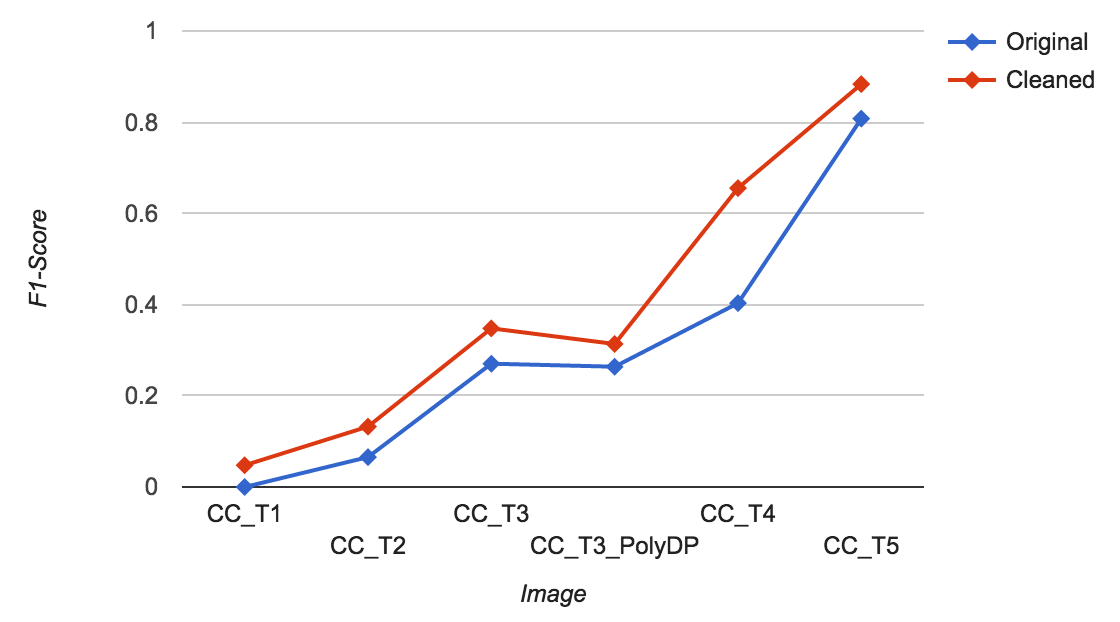
\includegraphics[width=1.0\textwidth]{CCF1ScoreGraphOCAverage}
	\caption{Averaged F1-Score of original (blue) and cleaned plans (red).}
	\label{fig:CCF1ScoreGraphOCAverage}
\end{figure}

Interesting is the difference in iteration 4 (\textit{CC\_T4}), because the cleaned floor plans have drastically increased their accuracy, but the original ones only marginally. This has to do with the false positive detection count. There is much more noise in the original plans, which leads to a higher count of false positives. Only when we increased the negative sample count to 1600, also the original plans could make a big step and double its accuracy.

The graph shows that it is recommended to do a clean up before processing the image. This includes removing unnecessary walls, furniture and markers.


\subsubsection{Gap closing}
\label{sub:GapClosing}
In this section, gap closing will be discussed. There are two different types of gap closing in this project. There is the outer-wall gap closing. This is mainly a gap closing of all the existing windows. This is important to circumvent the rooms to the outside of the house. The second part of gap closing is the door closing. It is important as per definition all rooms are separated by a door. By closing the door gap, the room finding algorithm will then be able to easily find each room.
\paragraph{Edge door closing}
The edge door closing algorithm was the first algorithm that was implemented to solve the problem of closing doors. The idea behind it was, that in the area of any found door with the cascade classifier, there would be a rectangle of corners that represent the edges of the walls where the door is attached to. Therefore, an algorithm was implemented, that detected those corners and then tested if there was an actual rectangle within that area.

The idea is that on the area a door is found there is usually no other rectangle of corners other than the door frame itself. This assumption is made after the morphological cleaning is done, therefore most noise that could have created a rectangle of corners should have been extinguished. On the image of the walls, the algorithm performs a Corner Detection (see section~\ref{subsubsec:HarrisCornerDetection}). This results in an image that represents all locations that are likely to be a corner with white pixels. Usually, one corner is detected in the form of several white pixels. To find the exact position of this corner the algorithm uses Point Clustering (see section~\ref{sec:PointClustering}) to find its center. After all corners and doors are found, the door gap closing algorithm (see section~\ref{sec:DoorGapAlgorithm}) kicks in. It finds the rectangles that create the door frame within the area of the detected door and some additional margins. This margin was added, as the detected door symbol usually does not contain the door frame and the wall enclosing it, and therefore does not have the corners within the original detection square.
When a door rectangle was found, it was filled with black color. This closed the gap on the image.

\begin{figure}[H]
	\centering
	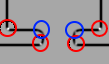
\includegraphics[width=0.6\textwidth]{CornerNotFound}
	\caption{This image shows the result of a corner detection. Blue circles represent corners that should have been found but were not. Red circles represent corners that were found by the Harris corner algorithm. In this image the door frame rectangle can not be found because two out of four corners are missing.}
	\label{fig:CornerNotFound}
\end{figure}

A big problem with this approach was, that some of the corners on floor plans were too round. As soon as one corner of the needed four was not detected the algorithm wouldn't close the gap. Additionally, if a wrongly detected door was enclosing a room within itself. The whole room was identified as a gap and therefore filled. This was a rare occurrence. This algorithm didn't deliver very good results,due to its very restrictive conditions.

\paragraph{Simple door closing}
\label{sub:SimpleDoorClosing}
As a result, an easier solution for gap closing was created. It again uses the squares with the location of the found doors. It makes use of the fact that on the image where all the noise was removed, the symbol of the detected door is erased. All that is left within the square, are walls. Due to the fact that the found door will always be where the gap for a door is, there have to be two ends to a wall as well. The algorithm connects those walls with a simple combination of erosion and dilation.

\begin{figure}[H]
	\centering
	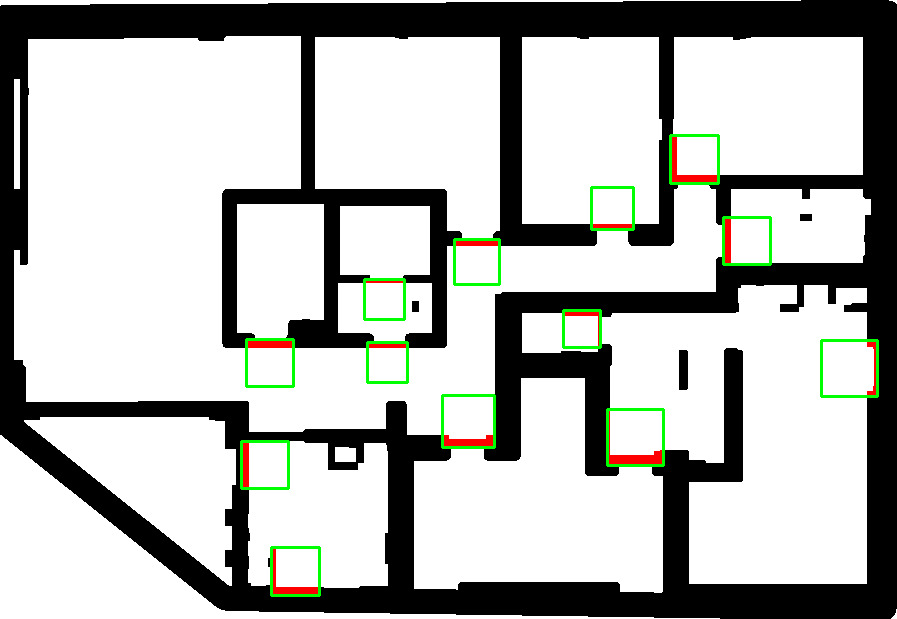
\includegraphics[width=1.0\textwidth]{SimplifiedGapClosingAN1}
	\caption{Simplified gap closing visualised on the plan AN\_1. The red areas represent the closed gaps.}
	\label{fig:SimplifiedGapClosingAN1}
\end{figure}

The lines of the wall within that square are eroded until they connect and then dilated back to their original size. The difference is that the gap is now filled and looks like it is part of the wall (Figure~\ref{fig:SimplifiedGapClosingAN1}). This algorithm doesn't have to deal with undetected corners. It will also not change any existing walls with no gaps that are within one of the squares. These walls will just be expanded and then resized to their original size. The only problem that was found with this algorithm, was that if the erosion size was too big, the whole square will be filled. This is obviously not intended and therefore incorrect.

\paragraph{Door closing comparison}
\ref{sec:DoorClosingComparison}
In this section both of the algorithms are compared to each other. It will describe how effective they were, and explain the results.

\begin{figure}[H]
	\centering
	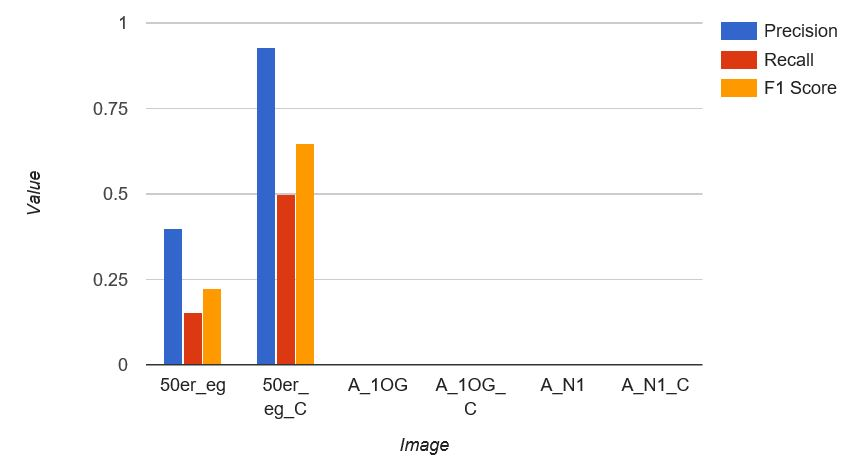
\includegraphics[width=1.0\textwidth]{pointDoorClosing}
	\caption{Precision, Recall and F1-Score for all images processed with the edge door closing algorithm. }
	\label{fig:pointDoorClosing}
\end{figure}

As shown in the figure \ref{fig:pointDoorClosing}, the images A\_1OG and A\_N1 do not have any scores at all. The problem for image A\_1OG is, that due to the structure of the doors within this plan, the algorithm can not find 4 corners to connect. The door frame is already closed, as the door symbol itself had a "wall" connecting the enclosing walls. The problem with the image A\_N1 is that there are never four edges detected for one door, because at least one of the supposed corners is too round. It is not detected as a corner and therefore no door closing is done. For the last plan, the cleaned version shows decent results, since the precision is at 90 percent. The problem is that not all doors are correctly detected and provide the four corners. Therefore the recall is only on 50 percent.

\begin{figure}[H]
	\centering
	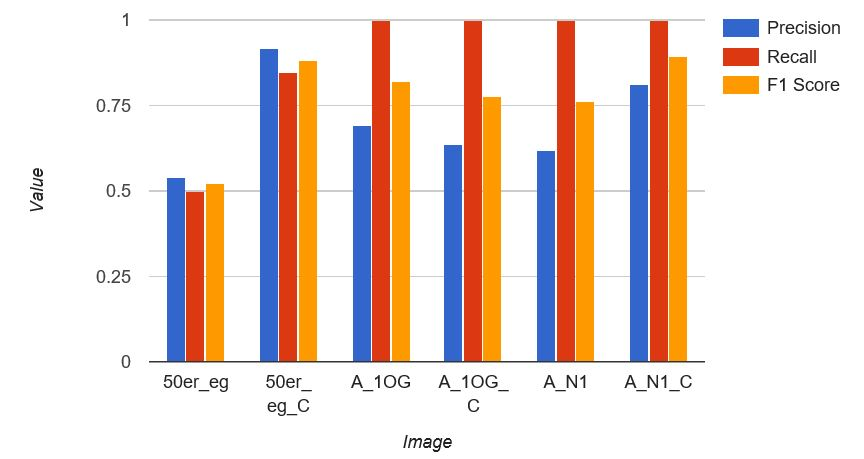
\includegraphics[width=1.0\textwidth]{simpleDoorClosing}
	\caption{Precision, Recall and F1-Score for all images processed with the simple door closing algorithm. }
	\label{fig:simpleDoorClosing}
\end{figure}

In comparison, the simple door closing algorithm shows much better results. The precision for all images is comparably low. This is due to the fact that the cascade classifier has identified more doors than are actually on the map. All of those additional found doors count as false positives. Important to note is that this does not impact the algorithm in a strong matter. Almost all of those false positives have no negative effect on the future algorithm as they usually draw over a present wall. This has no effect on the resulting image. This shows especially in the recall, where in two out of the three images all doors are closed.
For this door closing algorithm a good recall is the most important number as closing of false positives seldom real impact on the image itself.

As can be seen from the results of both of the algorithms, the second algorithm is a lot more robust to noise and like rounded corners and already closed doors. It does not need to identify any corners to work and closed doors are treated like a preexisting wall. This shows an extreme improvement for door gap closing on any image and has almost no drawbacks to our current knowledge. With the first algorithm, the implementation is very restricted to good conditions. The simple door closing algorithm in contrary will work under almost all circumstances and was therefore used for the final workflow.

\paragraph{Wall closing}
\label{sub:WallClosing}
As for wall closing, there were two different approaches tested. The most obvious approach was to find all the windows with object detection and then close those gaps. The problem with this attempt was, the way windows are represented in architectural floor plans changes on most plans. The few tests done showed very bad results and therefore it was decided that there had to be a different method to close the windows.

This new algorithm finds the outer walls by finding the convex hull for the polygon of the outside walls. It then closes them by drawing a line, that represents the closed wall, along the outer hull. This way, the outer bounds are all enclosed.
The algorithm will first find all the contours as described in section~\ref{sub:FindContoursTheory}. Based on those contours it will find the convex hull (see section~\ref{sub:ConvexHull}) of the outer polygon from all the drawn contours. This leads to the exact convex hulls of the outer walls. Sometimes there are outliers from the wall that have no connection to any room and would therefore create additional rooms. To try and prevent this, the polyDP (see section~\ref{sub:PolyDP}) was implemented. It can straighten out lines and therefore reject outliers of walls. This helped to create a more realistic outer wall.
\subsubsection{Room detection}
\label{sub:RoomDetection}
In the following section, the room detection used in the third workflow will be discussed. It features a short description the algorithm that was used for room detection and then discusses the different results.
\paragraph{Connected components}
\label{sec:ConnectedComponents}
To detect the rooms in workflow three the connected components algorithm was used. This algorithm is described in detail in section \ref{sub:ConnectedComponentAnalysis}. What it does is, that it creates groups of white pixels that are connected to each other. Each group of white pixels represents its own room. The connected component search is done after all noise removal, object detection and gap closing algorithms are run. An additional heuristic implemented is, that all rooms connected to the border of the image are not recognized as rooms. It is expected that any building has an outer wall, therefore no room can touch the border of the image.

In the figure \ref{fig:RoomDDResult}, the numbers for Precision, Recall and F1-Score for room detection with the connected components algorithm are listed. All of the tests were done by our team and a detailed description can be found in the file \textit{Evaluation.odf}, which comes with this work. Any information to replicate the tests can be found within this document. The tests resulting in this graph were done without any user interaction other than adjusting the algorithm parameters. There was no manual deletion of noise or closing of gaps by hand.

As seen in figure \ref{fig:RoomDDResult}, the results for the two uncleaned images are much worse than for the cleaned ones. This is due to the fact, that the outer wall closing does not work properly on an uncleaned image. This messes up most rooms, as a lot of windows are not closed. Unclosed windows create wrong rooms and have a negative effect on all three bench marks. The cleaned versions show a high precision with all of them being around 90 percent. This shows that the room detection works really good even without any user interaction. The high recall value shows, that no matter how complicated a plan is or how many rooms a plan has, that most of the rooms are still correctly detected. Any of these values can be further improved if the user takes more time to find better parameters for the algorithm. But these results should show a good representation of a daily detection, where the user will not take minutes to find the best possible parameter. Instead he will correct minor mistakes afterwards by hand, which is more time efficient.

\begin{figure}[H]
	\centering
	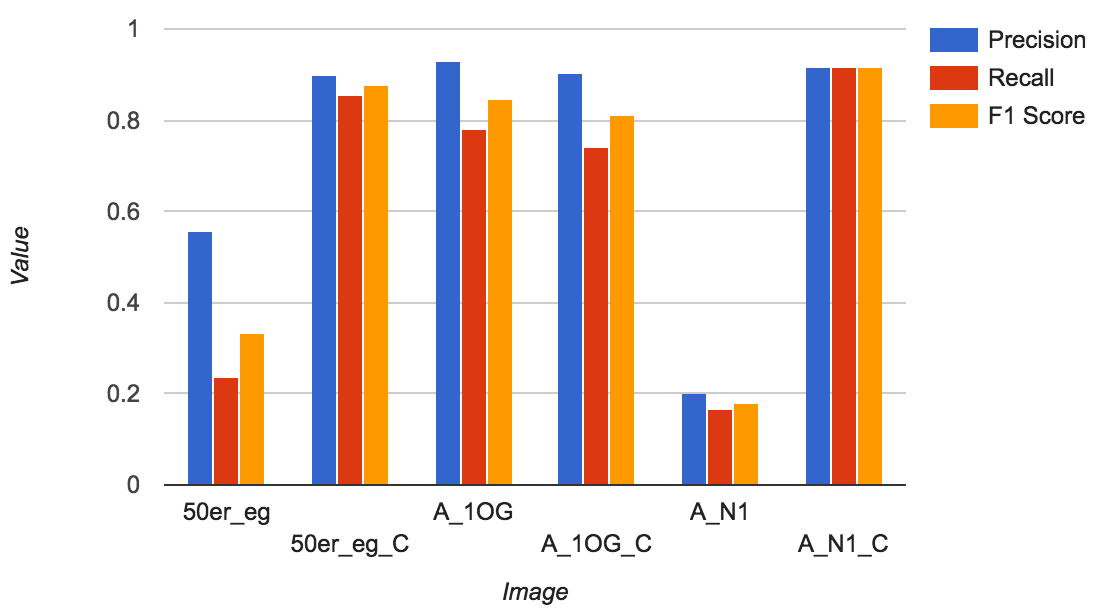
\includegraphics[width=1.0\textwidth]{RoomDDResult}
	\caption{This graph represents precision, recall and F1-score for all tested images. Each image was tested with an uncleaned and a cleaned version. The letter "C" represents that the image is the cleaned version. In the tests represented, there was no additional cleaning of the images with the tools available within the editor. }
	\label{fig:RoomDDResult}
\end{figure}

The following figure \ref{fig:RoomDDResult} shows the results of the same tests as the ones done above. The difference is, that in these tests the tester was able to use the tools provided within the editor. The figure shows a precision of a 100 percent. This improvement, especially in the uncleaned plans, was created due to the fact, that the editor can basically create a cleaned version of the plan. Therefore even the "uncleaned" versions show high precision and recall. If taken enough time, all those bench marks could be on a 100 percent, as you can basically redraw the plan with the existing tools. But those tests had to be done within a considerable amount of time. Therefore some of the plans do not have a recall of 100 percent.

\begin{figure}[H]
	\centering
	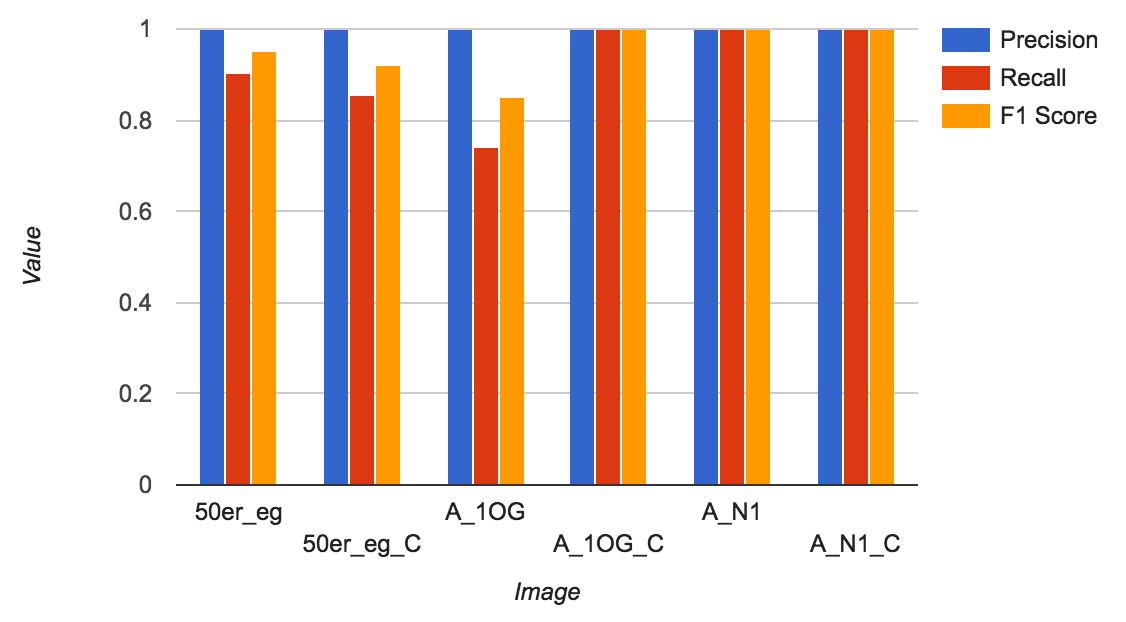
\includegraphics[width=1.0\textwidth]{RoomDDEResult}
	\caption{This graph represents precision, recall and F1-score for all tested images. Each image was tested with an uncleaned and a cleaned version. The letter "C" represents that the image is the cleaned version. In the tests represented, the tester did additional cleaning of the images with the tools available within the editor. These tools can create or erase lines. }
	\label{fig:RoomDDEResult}
\end{figure}

All of these bench marks discussed show how good the actual room detection works. But there is no comparison yet, what the improvements are compared to the old program used at the Planfabrik GmbH. As defined in the metrics, the whole process to detect the rooms was measured with clicks and time used to detect the rooms. This comparison with these values will be done just below.

As seen in figure \ref{fig:ClicksPerPlan}, the clicks or user input is far less, than the amount needed with the old program. This come from the fact, that algorithms finds the room corners directly and does not need one click per corner. As seen, the amount of clicks needed stays about the same for each detection run. This shows, that the user input will be about the same no matter how complicated or how many rooms a plan has. The clicks used are mostly to adjust the parameters for the algorithms. This is fare less than most plans have room corners on them. Additionally, most tests with cleaning done by the user take some more clicks. But it is within a very small margin, compared to the run with no error correction. What can be said about this program is, that it generally takes less clicks than the old program. Not only that, but the bigger the plan, the fewer additional clicks it takes to process compared to the old program. 

\begin{figure}[H]
	\centering
	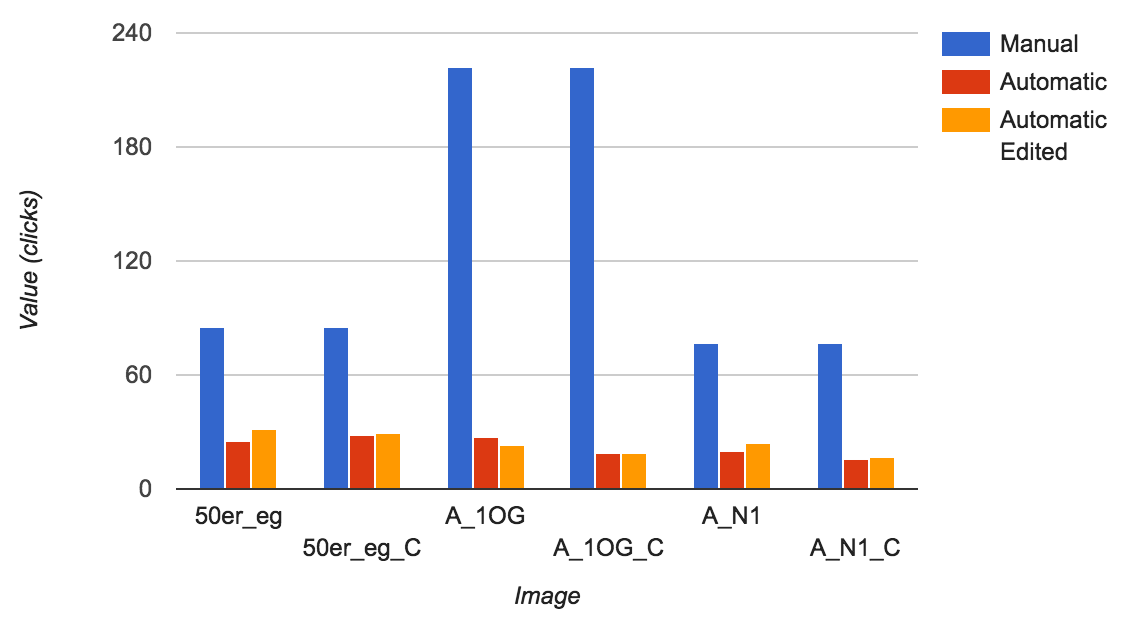
\includegraphics[width=1.0\textwidth]{ClicksPerPlan}
	\caption{This figure shows the clicks that were needed to fully process a plan. The blue bar represents the tests that were done with the old program within the Planfabrik GmbH. The red bar represents the tests without user editing of plans, while the orange bar represents wit user editing.}
	\label{fig:ClicksPerPlan}
\end{figure}

The same as in figure \ref{fig:ClicksPerPlan} was done in figure \ref{fig:TimePerPlan}. The difference is that figure \ref{fig:TimePerPlan} shows the time instead of the clicks needed. This graph indicates the same results as the other graph. It takes more time to find the rooms on a bigger plan when done with the old program. This program shows only small differences in time consumed, no matter the difficulty of the plan that was tested. 

\begin{figure}[H]
	\centering
	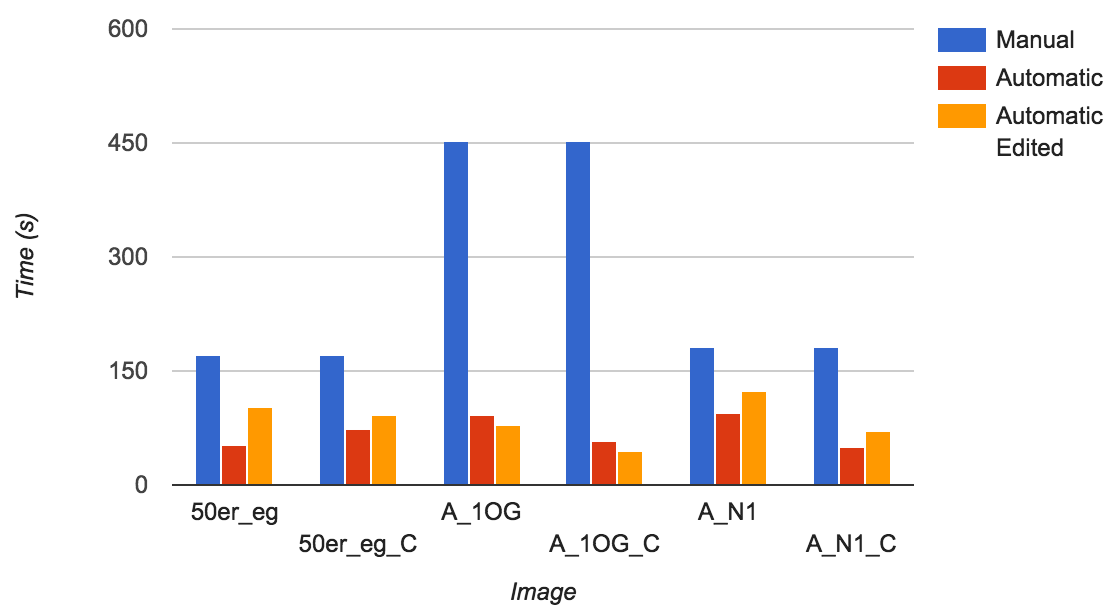
\includegraphics[width=1.0\textwidth]{TimePerPlan}
	\caption{This figure shows the time that was needed to fully process a plan. The blue bar represents the tests, that were done with the current process within the Planfabrik GmbH. The red bar represents the tests without user editing of plans, while the orange bar represents with user editing.}
	\label{fig:TimePerPlan}
\end{figure}

In general we can say, that this algorithm does solve the problem faster and with less user interaction than the old program.

\paragraph{Minimum room deletion}
\label{sub:MinimumRoom}
To improve the actual room detection, a simple heuristic was created. The problem was, that due to the fact that the wall closing algorithm was not perfect and other factors, very small rooms were detected, that were no rooms. This was so obvious that those detected rooms could not be a room itself, because they were more than a hundred times smaller than the biggest room.
To reject these rooms the program provides a factor, usually one percent, that the rooms to be removed have to be smaller than the biggest room of the house. This one percent is calculated on the area of both rooms and it is a measure that proved to be solid for all tested plans.

\paragraph{Result}
To test how accurate the room detection works, we analysed a floor plan and compared the results of the software with the values, which are stated on the actual plan. The test uses the plan \textit{50er} and \textit{50er\_C} and its \textit{BF} (\textit{Boden Fläche}) label as room size.

\begin{figure}[H]
	\centering
	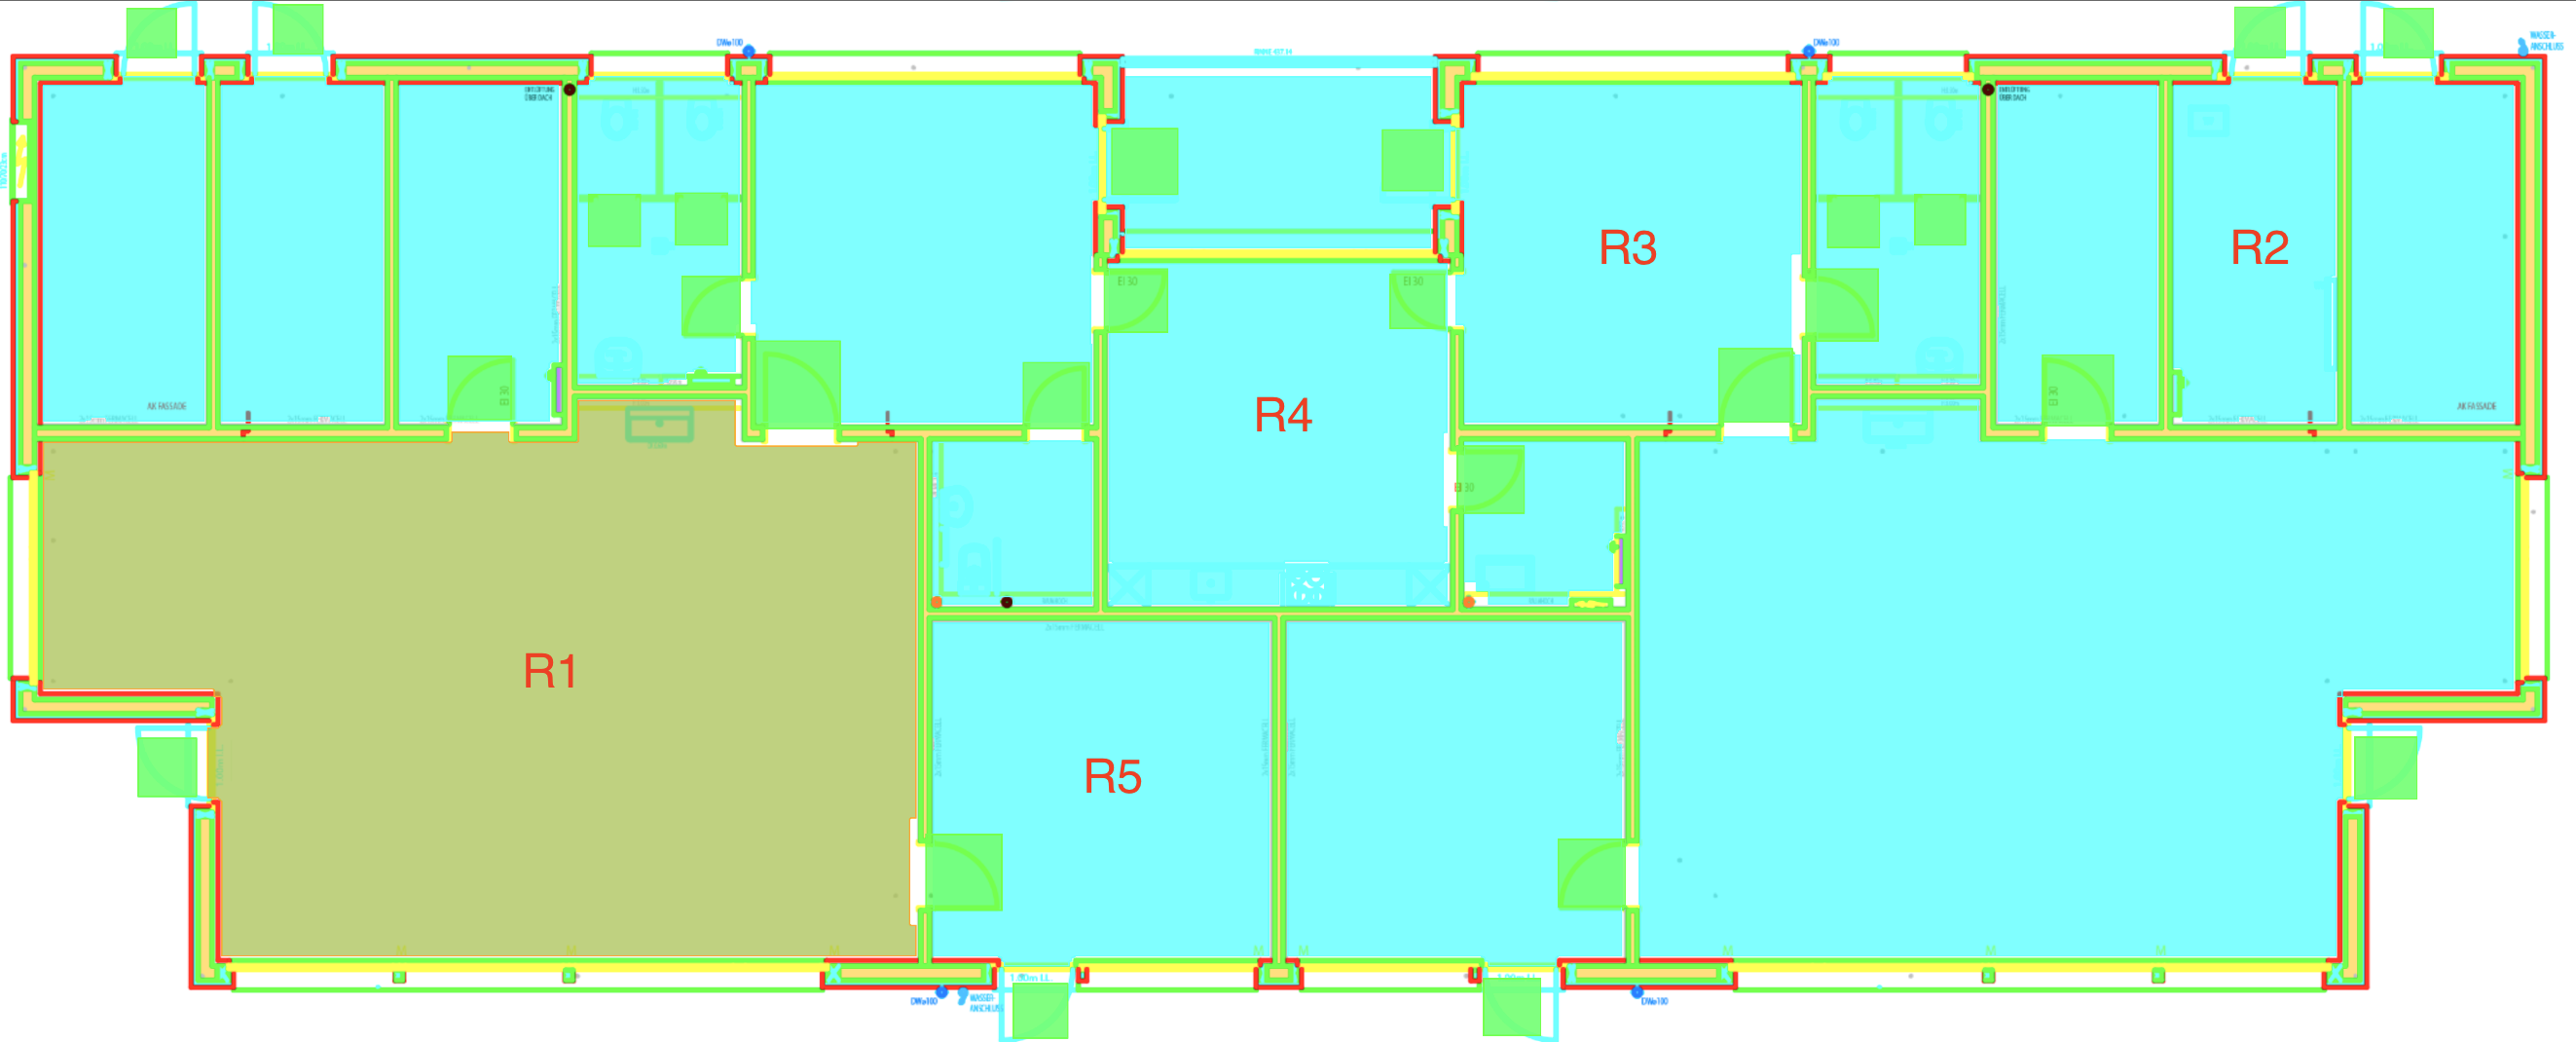
\includegraphics[width=1.0\textwidth]{50erRoomSize}
	\caption{This figure shows the 50er\_C room plan with the marked room polygons. For the accuracy test, the red marked rooms are used.}
	\label{fig:50erRoomSize}
\end{figure}

Only five of the rooms have been tested, because most of the rooms have the same size. We tried to use different room sizes to get a representative result of the accuracy. The rooms are marked in figure~\ref{fig:50erRoomSize} with a red label. The test was done with default small edits by the user, to simulate a real workflow.

\begin{figure}[H]
	\centering
	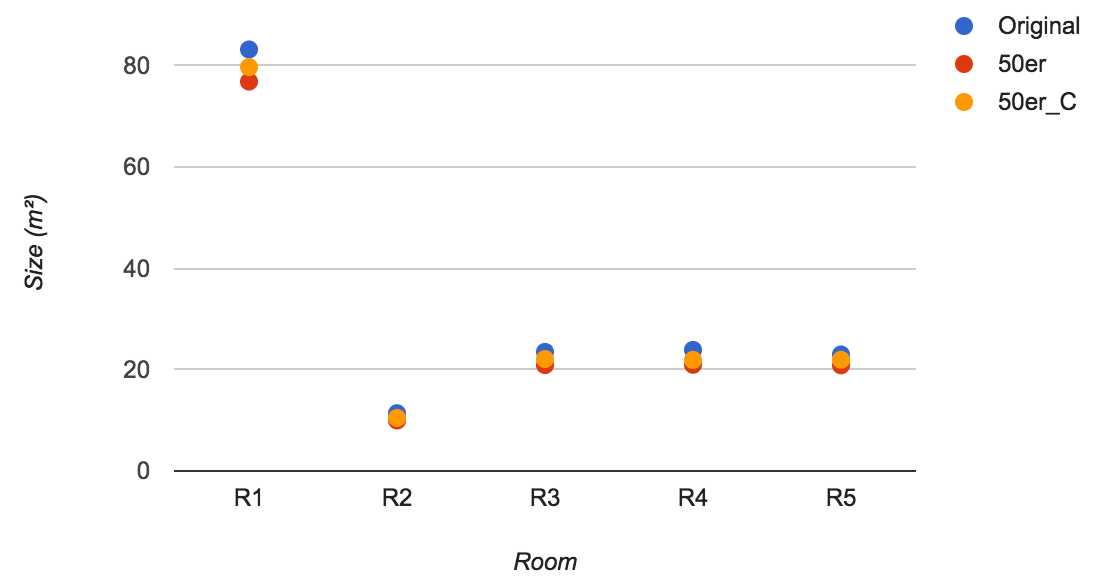
\includegraphics[width=1.0\textwidth]{50erRoomAccuracy}
	\caption{This figure shows the accuracy test results of the 50er\_C room plan in $m^{2}$.}
	\label{fig:50erRoomAccuracy}
\end{figure}

As shown on figure~\ref{fig:50erRoomAccuracy}, the detected room sizes are always smaller then the actual values. The larger the room, the bigger is the deviation in m$^{2}$. We think this is, because the algorithm is missing some areas at the doors and because of the inaccuracy of the ruler tool. With this tool, it is possible to set the distance relations and if this is done inaccurate, all room sizes will suffer from it.

\begin{figure}[H]
	\centering
	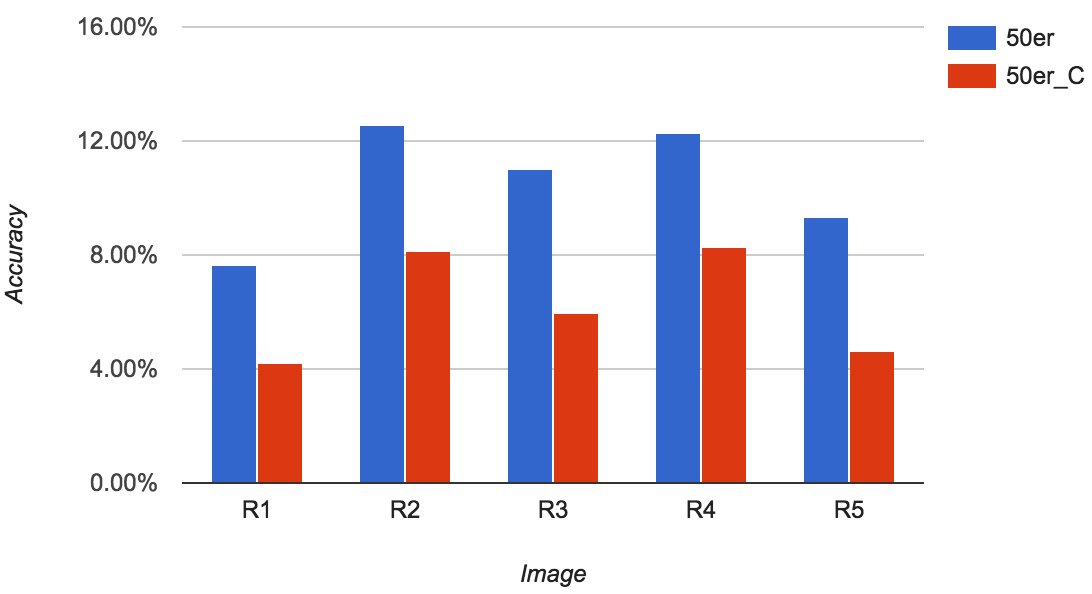
\includegraphics[width=1.0\textwidth]{50erRoomAccuracyPercent}
	\caption{This figure shows the accuracy test results of the 50er\_C room plan in percent.}
	\label{fig:50erRoomAccuracyPercent}
\end{figure}

The deviation is even stronger on original plans than on cleaned plans (Figure~\ref{fig:50erRoomAccuracyPercent}). We think this comes from the fact, that the cleaned plans have less noise on it, which could create interferences in the room polygons.

Our test showed that there is an average deviation of 10.55percent on original plans and 6.25 percent on cleaned floor plans.


